\section{The \igh{} locus of \nfu}
\label{sec:nfu-locus}

\subsection{Assembling the \Nfu \igh{} locus}
\label{sec:nfu-locus-assembly}

In order to locate and characterise the \nfu \igh{} locus, databases of \vh, \jh, and \ch exon sequences were collated from the published locus sequences of three reference species (zebrafish \parencite{danilova2005zebrafish}, three-spined stickleback \parencite{bao2010stickleback,gambondeza2011stickleback}, and medaka \parencite{magadan2011medaka}) and aligned to the \nfu genome (NFZ2.0) with \program{BLAST} \parencite{altschul1990blast,altschul1997blast}. Genome scaffolds with high-confidence alignments to at least two distinct segment types or covering at least 1\% of the scaffold's total length were retained for downstream analysis as potential locus candidates. In total, one chromosome (chr6) and 6 unincorporated scaffolds were identified as potentially covering part of the locus sequence (\Cref{tab:nfu-locus-scaffolds}), with chromosome 6 bearing the majority of identified gene segments.  %TODO: Add genome accession when available

\begin{table}[bh]
\centering
\caption{\Nfu genome scaffolds containing putative \igh{} locus fragments.}
\begin{threeparttable}
\begin{tabular}{cccccccc}\toprule
\textbf{Scaffold} & \textbf{Total length (kb)} & \textbf{V} & \textbf{J} & \textbf{\cm{}} & \textbf{\cd{}} & \textbf{\cz{}} & Included in locus?\\\midrule
chr6 & 6195.6 & 15 & 7 & 5 & 11 & 0 & Yes\\\midrule
scf10901 & 1.4 & 0 & 0 & 0 & 3 & 0 & Yes\\
scf21863 & 13.5 & 1 & 0 & 0 & 0 & 0 & No\\
scf35954 & 16.3 & 3 & 0 & 0 & 0 & 0 & No\\
scf36277 & 18.9 & 2 & 1 & 0 & 0 & 0 & No\\
scf37083 & 17.7 & 1 & 0 & 0 & 0 & 0 & No\\
scf9157 & 7.2 & 0 & 7 & 4 & 0 & 0 & Yes\\\bottomrule
\end{tabular}

\end{threeparttable}
\label{tab:nfu-locus-scaffolds}
\end{table}

\begin{table}[bh]
\centering
\caption{\Nfu BAC-library inserts containing putative \igh{} locus fragments.}
\begin{threeparttable}
\begin{tabular}{cccccccc}\toprule
\textbf{BAC ID} & \textbf{Insert length (kb)} & \textbf{V} & \textbf{J} & \textbf{\cm{}} & \textbf{\cd{}} & \textbf{\cz{}} & Included in locus?\\\midrule
154G24 & 106.6 & 17 & 1 & 0 & 0  & 0 & No\\
162F04 & 119.4 & 5  & 1 & 0 & 0  & 0 & No\\
165M01 & 110.7 & 15 & 1 & 0 & 0  & 0 & Yes\\
206K13 & 106.7 & 17 & 1 & 0 & 0  & 0 & No\\
208A08 & 103.2 & 17 & 1 & 0 & 0  & 0 & Yes\\
209K12 & 133.0 & 1  & 8 & 4 & 20 & 0 & Yes\\
220O06 & 104.8 & 4  & 1 & 0 & 0  & 0 & No\\
223M21 & 99.3  & 17 & 1 & 0 & 0  & 0 & No\\
248A22 & 47.3  & 7  & 0 & 0 & 0  & 0 & No\\
276N03 & 127.9 & 7  & 0 & 0 & 0  & 0 & Yes\\
277J10 & 120.8 & 17 & 1 & 0 & 0  & 0 & Yes\\
\bottomrule\end{tabular}

\end{threeparttable}
\label{tab:nfu-locus-bacs}
\end{table}

In order to determine which of the putative locus scaffolds were in fact part of the \igh{} locus, integrate these into a contiguous locus sequence, and provide additional information on any missing gene segments, bacterial artificial chromosome insert sequences from the killifish genome project BAC library \parencite{reichwald2015genome} were included in the locus assembly. BAC candidates, whose ends had already been sequenced as part of the genome project, were identified as potentially containing part of the locus sequence on the basis of their ends aligning to promising candidate scaffolds from a previous genome assembly (first round) or to the insert sequences of previously sequenced BAC inserts (second round). Once identified,  BAC candidates were isolated from culture by alkaline lysis, sequenced on an Illumina MiSeq sequencing machine, and assembled and scaffolded with \program{SPAdes} and \program{SSPACE}, respectively. Complete BAC insert assemblies were generated from these scaffolds by manual alignment to overlapping genome scaffolds and other BAC inserts, combined with PCR and Sanger sequencing of intervening sequences.

Finally, the assembled BAC inserts were screened for \igh{} locus segments in the same manner described for genome scaffolds, and passing insert sequences (\Cref{tab:nfu-locus-bacs}) were aligned to and integrated with the identified candidate scaffolds to produce a contiguous locus assembly. To minimise the probability of losing relevant gene segments to assembly errors, priority in the event of a sequence conflict between BACs and scaffolds was given first to any sequence containing a segment missing from the other; if neither the BAC assembly nor the genome scaffolds met this condition, priority was given to the genome scaffold over the BAC assembly. In total, 3 candidate scaffolds (including chromosome 6) and 5 BAC inserts were included in the final locus assembly, while 4 scaffolds and 6 BACs were excluded as likely representing isolated \igh{} orphon segments elsewhere in the genome. The correspondence between the final locus sequence and the sequences used to construct it is shown in \Cref{fig:nfu-locus-aln}.

\begin{figure}
\centering
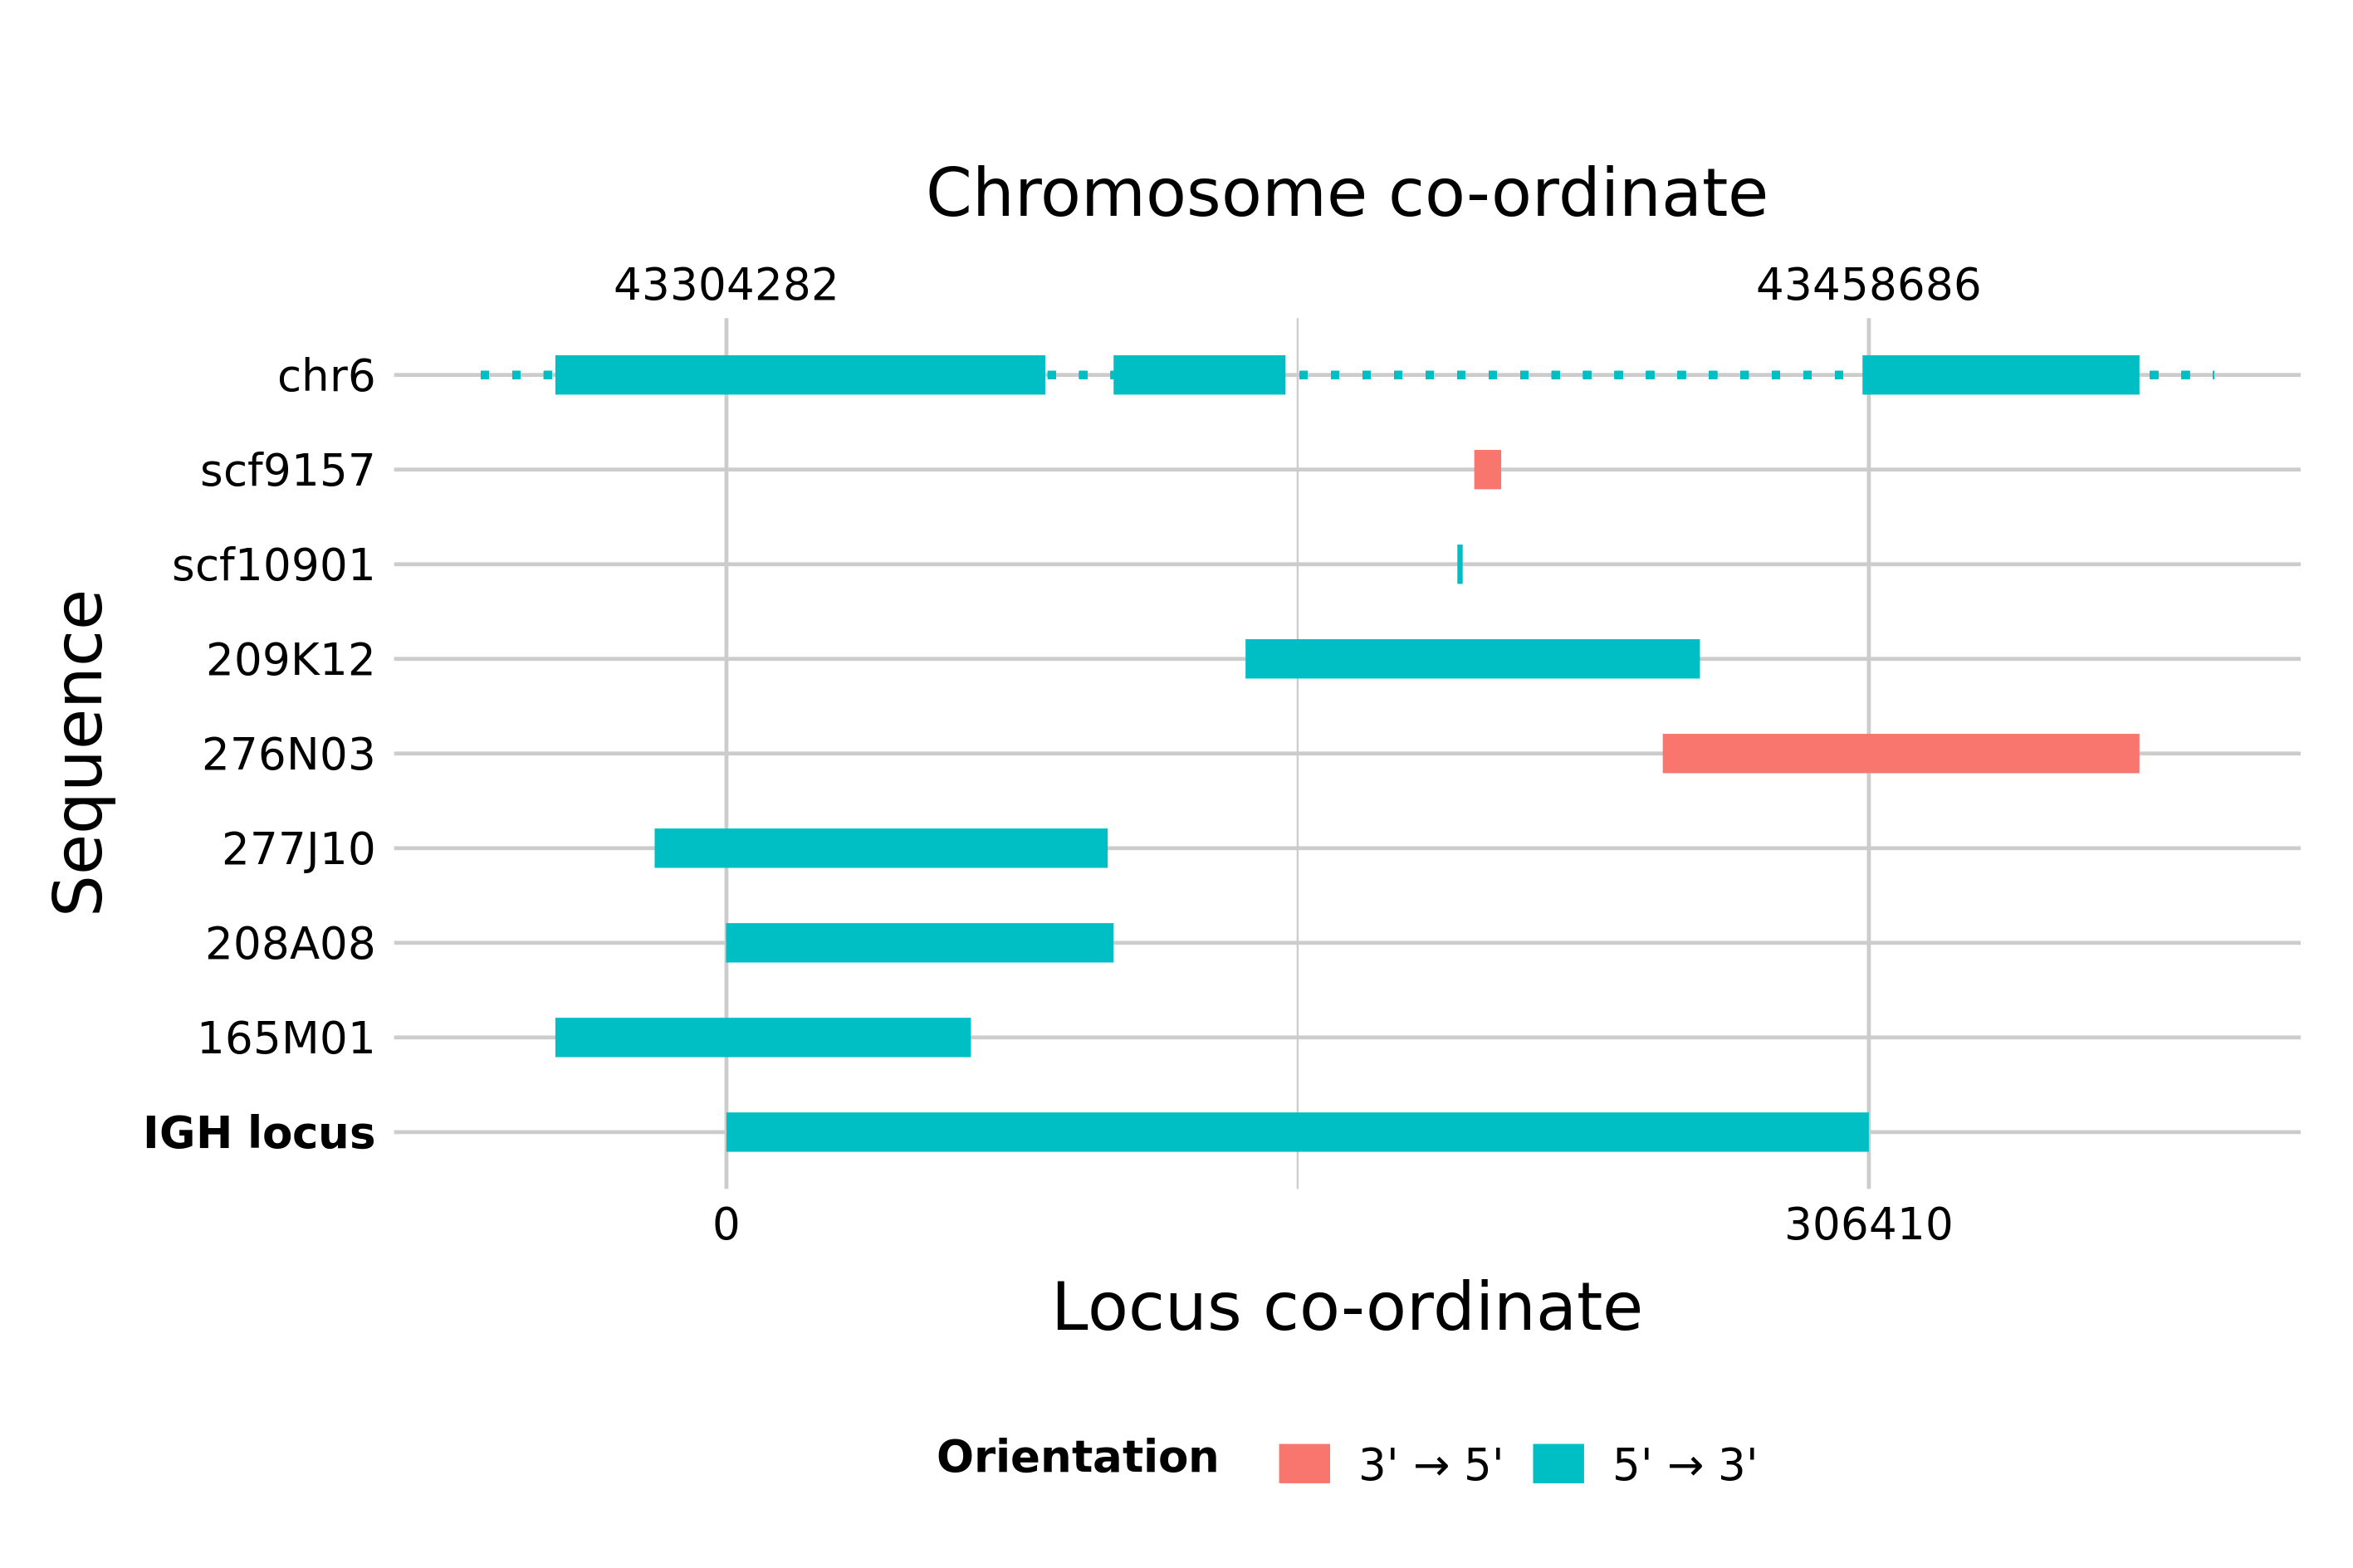
\includegraphics[width=\textwidth]{_Figures/png/nfu-locus-aln}
\caption[Assembling the \Nfu \igh{} locus]{\textbf{Assembling the \Nfu \igh{} locus:} Schematic of genome scaffolds and BAC inserts contributing to the \Nfu \igh{} locus sequence, with their corresponding place within the locus sequence (bottom axis). Internal gaps with dotted lines indicate locus regions with no corresponding locus sequence, as a result of intercalation of BAC or scaffold sequences.}
\label{fig:nfu-locus-aln}
\end{figure}

\subsection{Overall locus structure}
\label{sec:nfu-locus-structure}
	
The turquoise killifish genome contains a single \igh{} locus approximately 306 kilobases in length, located on chromosome 6 of the \Nfu genome (\Cref{fig:nfu-locus-map-a}). This locus comprises two complete subloci, \igh{1} (\kb{155}) and \igh{2} (\kb{118}), present in tandem and each occupying a classic {\vh-\dh-\jh-\ch} translocon configuration. This modified translocon structure, with multiple translocon subloci present in tandem, has been observed in a number of teleost \igh{} loci including catfish, medaka and stickleback \parencite{fillatreau2013astonishing}. Unusually, however, the smaller \igh{2} sublocus in \nfu \igh{} is present in antisense relative to the larger \igh{1}, with the two subloci beginning at opposite ends of the locus and facing each other in the middle (\Cref{fig:nfu-locus-map-b}). Such a multi-orientation locus structure has only previously been observed in medaka, the closest relative of the turquoise killifish to have its locus characterised prior to the present study \parencite{magadan2011medaka}; it is interesting to see this unusual feature reproduced here, raising the question of whether that this ideosyncracy is homologous between the two loci.
	
Compared to other closely-related loci, the killifish locus is relatively sparse and simple, with comparatively low functional complexity relative to its overall size. For example, whereas the stickleback locus fits four subloci, 49 V segments and 10 constant regions into c. \kb{200} \parencite{bao2010stickleback,gambondeza2011stickleback}, the killifish locus, despite being ~50\% longer, contains only 2 subloci, four constant regions and 24 V segments (including pseudogenised Vs). This difference results from the unusually large amount of nonfunctional sequence padding the killifish locus, resulting in large gaps between variable segments and in some cases between constant-region exons (\Cref{fig:nfu-locus-map-b}); this high prevalence of repetitive DNA is consistent with the rest of the turquoise-killifish genome, which comprises more than 60\% repetitive sequence \parencite{willemsen2019popgen}, compared to just over 15\% in stickleback \parencite{yuan2018repeats}. % TODO: Reference for Nfu repeat level - Cui et al ...
	
The two subloci in the turquoise killifish locus are generally highly similar in their functional sequence, with a high degree of synteny between their functional regions (\Cref{fig:nfu-locus-synteny}). The greatest degree of divergence occurs in the \vh and \dh regions, with what appear to be repeated deletion events in IGH2 resulting in a substantially lower number of \vh and \dh segments compared to IGH1; conversely, the \jh and constant regions are almost identical between two subloci. These patterns are discussed in more detail in \Cref{sec:nfu-locus-constant,sec:nfu-locus-variable}.
	
\begin{figure}
	\centering
	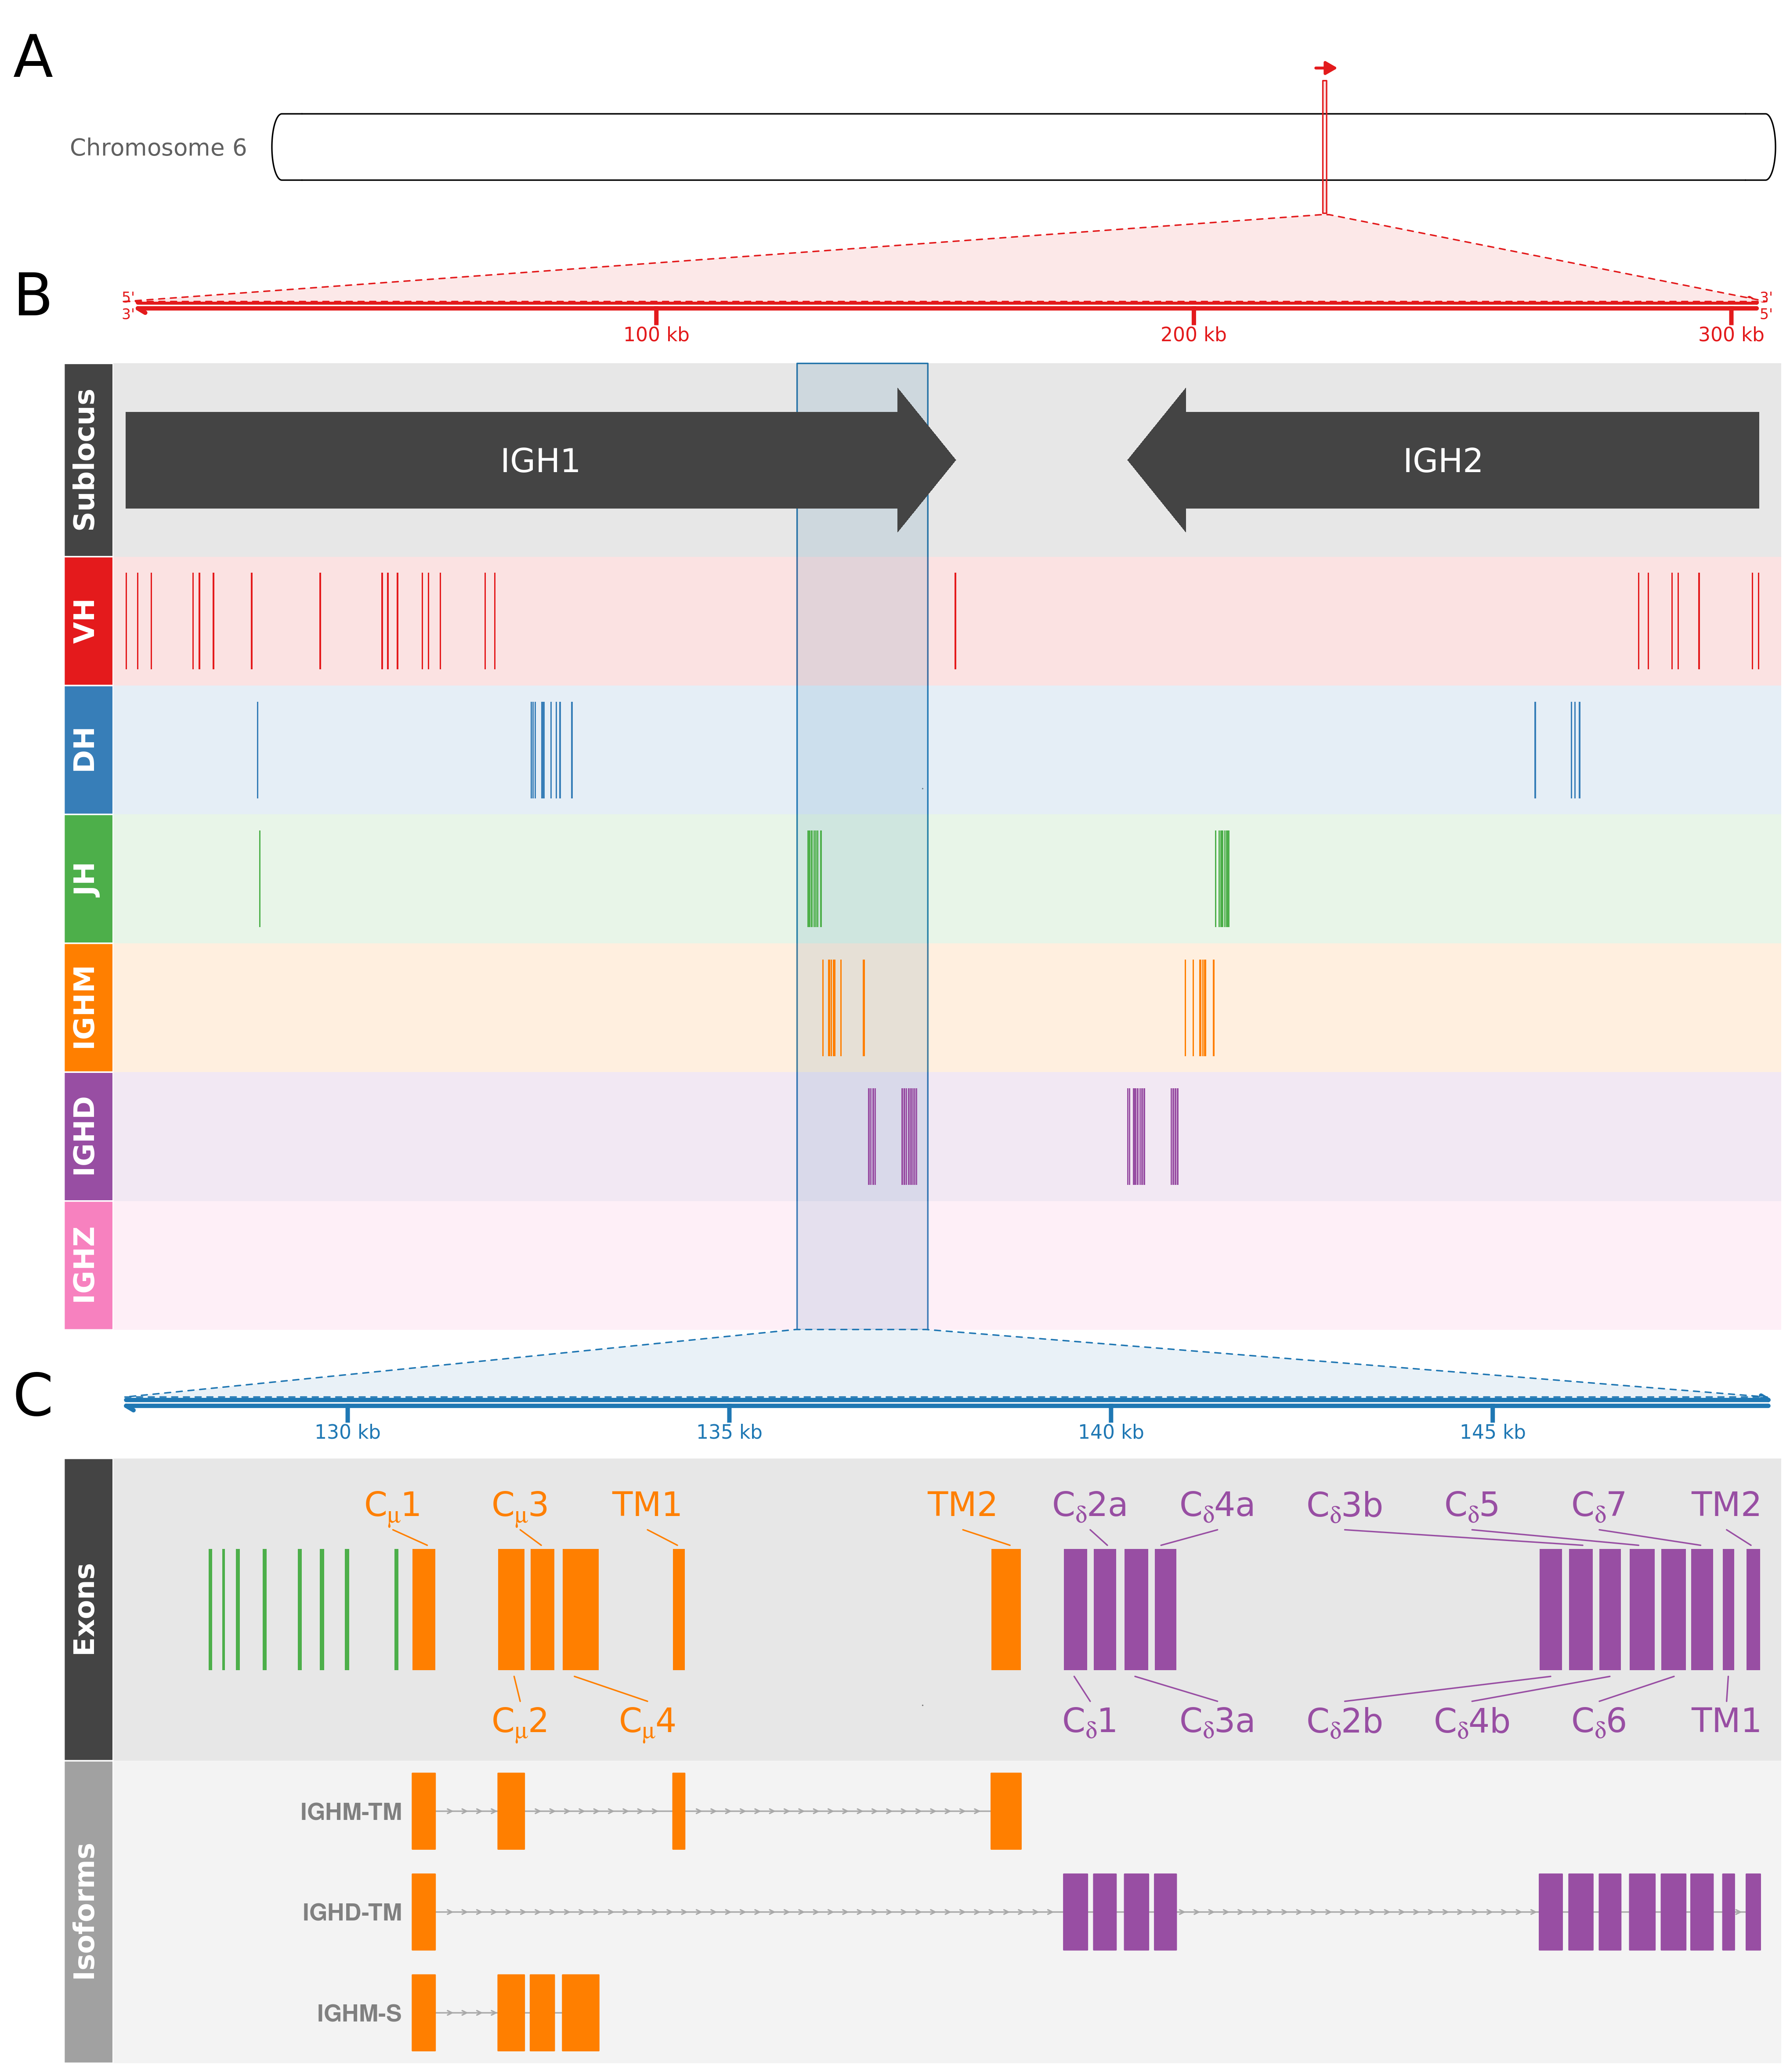
\includegraphics[width=\textwidth]{_Figures/png/nfu-locus-map}
			    \begin{subfigure}{0em}
        \phantomsubcaption{}
        \label{fig:nfu-locus-map-a}
    \end{subfigure}
    \begin{subfigure}{0em}
        \phantomsubcaption{}
        \label{fig:nfu-locus-map-b}
    \end{subfigure}
    \begin{subfigure}{0em}
        \phantomsubcaption{}
        \label{fig:nfu-locus-map-c}
        \end{subfigure}
	\caption[The immunoglobulin heavy chain (\igh{}) locus in \nfu]{\textbf{The immunoglobulin heavy chain (\igh{}) locus in \nfu:} (A) Position of the \igh{} locus on chromosome 6 of the \Nfu genome. (B) Arrangement of \vh, \dh, \jh and constant-region gene segments on the \Nfu \igh{} locus. All segments follow the orientation of their parent sublocus, indicated in the uppermost track. (C) Detailed map of the constant regions of the \textit{IGH1} sublocus, indicating the position and identity of the constant-region exons and the exon composition of expressed \igh{} isoforms in the turquoise killifish.}
	\label{fig:nfu-locus-map}
	\end{figure}
	
\begin{figure}
	\centering
	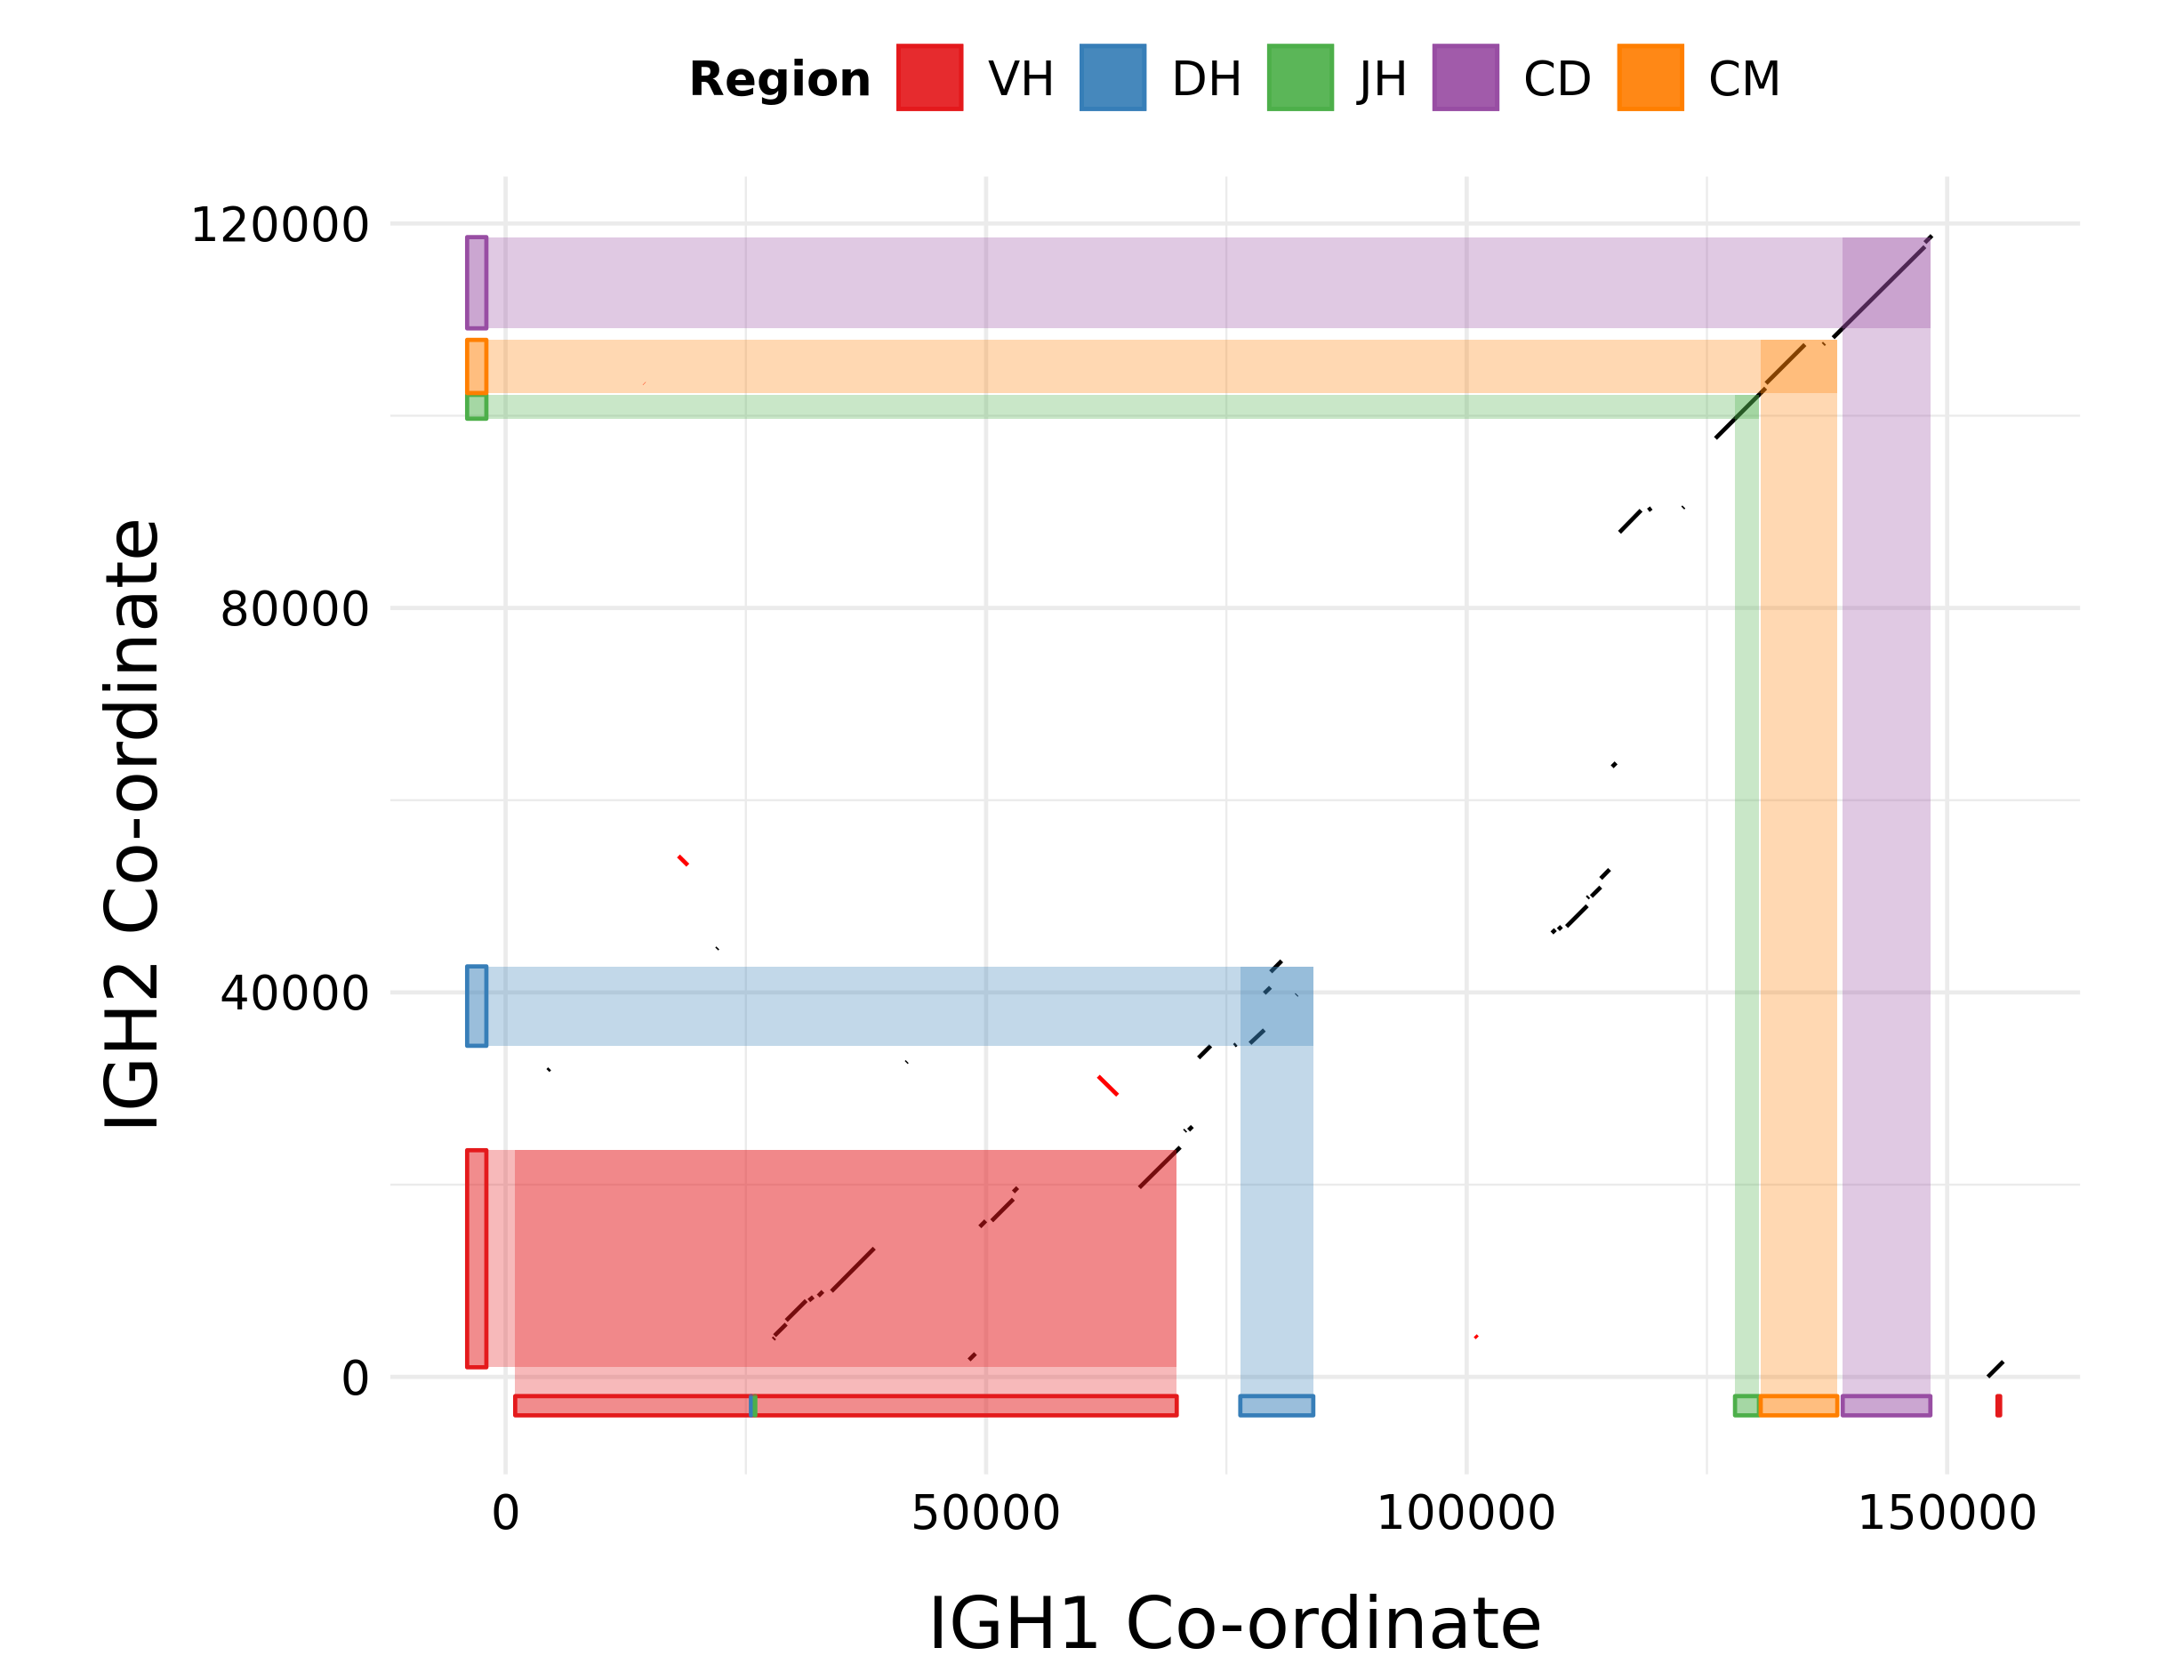
\includegraphics[width=0.9\textwidth]{_Figures/png/nfu-locus-dots}
	\caption[Sequence homology between subloci in \Nfu \igh{}]{\textbf{Sequence homology between subloci in \Nfu \igh{}:} Synteny plot of sequential best matches between \igh{1} and \igh{2} subloci, with gene segment regions indicated by coloured rectangles along each axis.}
	\label{fig:nfu-locus-synteny}
\end{figure}
	
	\subsection{Constant regions}
	\label{sec:nfu-locus-constant}

\newabbreviation{IGHM-S}{IGHM-S}{secretory IGHM}
\newabbreviation{IGHM-TM}{IGHM-TM}{transmembrane IGHM}
\newabbreviation{NT}{NT}{nucleotide(s)}
\newabbreviation{AA}{AA}{amino acid(s)}
\newabbreviation{nt}{nt}{nucleotide(s)}
\newabbreviation{mRNA}{mRNA}{messenger RNA}

	
	The \textit{isotype} (also known as the \textit{class}) of an antibody determines its functional role within the immune system, including its possible effector functions and whether it can be secreted \parencite{schroeder2010immunoglobulins}. Three antibody isotypes have been identified to date in teleost fishes: \igh{M}, \igh{D} and \igh{Z} (a.k.a. \igh{T}, \igh{T/Z} or \igh{Z/T}) \parencite{fillatreau2013astonishing,bengten2015fishantibodies,magadan2015fishrepertoires}. Of these, \igh{M} and \igh{D} are highly primitive within the jawed vertebrates and found in most or all other vertebrate groups; within the teleosts, both appear to be universal \parencite{bengten2015fishantibodies}. Conversely, \igh{Z} is a teleost-specific isotype which is absent in other vertebrate taxa; within the teleosts, most characterised \igh{} loci possess \igh{Z}, but at least two (medaka and channel catfish) have been found to lack it \parencite{fillatreau2013astonishing,bengten2015fishantibodies}. In rainbow trout, \igh{Z} has been found to play a specialised mucosal role in the immune system analagous to that of \igh{A} in mammals \parencite{zhang2010igtgut,xu2013igtskin}, and it is widely assumed to play this specialised role throughout the teleosts; it is as yet unclear how mucosal immunity is effected in species lacking \igh{Z}.
	
	In order to investigate constant regions in the \nfu \igh{} locus, putative exon sequences were identified using \program{BLAST} alignments to the reference sequence databases described in \Cref{sec:nfu-locus-assembly}, and intron/exon bounderies were refined through alignment of published RNA-sequencing data from killifish gut (\parencite{smith2017microbiota}, BioProject accession PRJNA379208, young and old untreated groups) using \program{STAR} \Cref{fig:nfu-locus-sashimi}. Strikingly, the \nfu \igh{} locus appears to completely lack any \igh{Z} constant region, with no \cz{} exons or \igh{Z} transmembrane exons being found on either \igh{1} or \igh{2}. Given the widespread prevalence and specialised mucosal role of \igh{Z} in teleosts, its surprising absence in turquoise killifish (\Cref{fig:nfu-locus-map-b}) immediately raises questions about the nature, kinetics and efficacy of mucosal adaptive immunity in this species. The similar absence of \igh{Z} in medaka, which again is the closest relative of \Nfu with a characterised locus, raises further questions about the evolutionary history of \igh{Z} in the Atherinomorpha: does the shared absence of \igh{Z} in these species indicate a single ancestral deletion event, or parallel loss of this important isoform within both the Cyprinodontiformes (including the turquoise killifish) and Beloniformes (including medaka)? This latter question requires higher phylogenetic resolution to address effectively, and is investigated further in \Cref{sec:xma-locus} and \Cref{sec:comparative}.
	
	While \igh{Z} is completely missing from the \Nfu \igh{} locus, \igh{M}, the most primitive and widely-found isotype in jawed vertebrates, is present in its expected location, immediately downstream of the main \jh-region in both subloci. This constant region occupies the standard six-exon configuration, with four \cm{} exons and two transmembrane exons present in series on the chromosome (\Cref{fig:nfu-locus-map-b,fig:nfu-locus-map-c,fig:teleost-igm-exons-a}, \Cref{tab:nfu-ch-coords}). As with other species, both secreted and transmembrane isoforms of \igh{M} are present in the transcriptome, with secreted \igh{M} (\igh{M-S}) consisting of \cm{1-4} (\Cref{fig:nfu-locus-map-c,fig:nfu-locus-sashimi-a,fig:teleost-igm-exons-b}); however, the exon configuration of transmembrane \igh{M} (\igh{M-TM}) deviates from both that seen in mammals (in which exon TM1 is spliced to a cryptic splice site within \cm{4}) and most teleosts (in which the canonical splice site following \cm{3} is used and \cm{4} is excised) \parencite{fillatreau2013astonishing}. Rather, turquoise-killifsh \igh{M-TM} resembles that of medaka, in which both \cm{3} and \cm{4} are excluded and the canonical splice site at the end of \cm{2} is spliced directly to TM1 (\Cref{fig:teleost-igm-exons-c,fig:teleost-igm-exons-d,fig:teleost-igm-exons-e}). This similarity to medaka again raises the possibility that this unusual feature may be a conserved feature of both lineages; however, the underlying mechanism giving rise to this difference in splicing behaviour is unknown.
	
		Unlike \igh{M}, the exon structure of \igh{D} is highly variable across the teleosts, ranging from roughly 7-17 \cd{} exons in addition to the transmembrane domains \parencite{fillatreau2013astonishing}. The core structure of \igh{D} comprises seven \cd{} exons (\cd{1-7}), but some subset of these exons may be missing or duplicated in any given species -- in medaka, for example, \cd{5} is missing in all subloci \parencite{magadan2011medaka}, while in many species (e.g. zebrafish, salmon, and channel catfish) \cd{2-4} are duplicated in two or more tandem blocks \parencite{fillatreau2013astonishing}. This latter configuration is also observed in turquoise killifish, in which the \igh{D} constant region immediately follows \igh{M} in both subloci and has a 

\cd{1}-(\cd{2}-\cd{3}-\cd{4})$_2$-\cd{5}-\cd{6}-\cd{7}-TM1-TM2 

	\noindent configuration, for a total of 12 exons per \igh{D} constant region (\Cref{fig:nfu-locus-map-b,fig:nfu-locus-map-c}, \Cref{tab:nfu-ch-coords}). All of these exons appear to be expressed in tandem, resulting in a much longer transcript than is observed for any isoform of \igh{M} (\Cref{fig:nfu-locus-map-c,fig:nfu-locus-sashimi-b}). As in other teleost species, \igh{D} in the turquoise killifish includes a chimeric \cm{1} exon at the 5' end of the constant-region transcript, for a total of 13 exons per \igh{D-TM} mRNA (\Cref{fig:nfu-locus-sashimi-b}).

	While the best-known form of \igh{D} in teleosts is transmembrane, secreted \igh{D} has been observed in at least two teleost species, with different mechanisms used in each case: in channel catfish, one dedicated sublocus has a dedicated \igh{D} secretory exon in place of the transmembrane exons \parencite{bengten2006catfish}, while in rainbow trout (and possibly some other species like Atlantic salmon and cod) a run-on event at the end of \cd{7} results in the production of a secretory tail in a manner similar to secretory \igh{Z} \parencite{ramirezgomez2012secretoryigd}. However, neither a specialised secretory exon nor a \cd{7} secretory tail could be detected in turquoise killifish, suggesting that \igh{D} may only be expressed in transmembrane form in this species.
	
	In the case of both \igh{M} and \igh{D}, the constant regions are present in their expected configuration in each sublocus and are highly similar in sequence between the subloci, with an average of 98.4\% nucleotide sequence identity for corresponding \igh{M} exons and 99.3\% for corresponding \igh{D} exons (\Cref{fig:nfu-ch-aln} and \Cref{tab:nfu-ch-aln}) in pairwise Needleman-Wunsch alignments \parencite{needleman1970align}. This high level of similarity indicates either a very recent duplication event to produce the second sublocus or a high level of sequence conservation in both subloci, with the latter explanation suggesting that both subloci continue to be functional and active in the immune system.
	
	\begin{figure}
	\centering
		    \begin{subfigure}{0em}
        \phantomsubcaption{}
        \label{fig:teleost-igm-exons-a}
    \end{subfigure}
    \begin{subfigure}{0em}
        \phantomsubcaption{}
        \label{fig:teleost-igm-exons-b}
    \end{subfigure}
    \begin{subfigure}{0em}
        \phantomsubcaption{}
        \label{fig:teleost-igm-exons-c}
    \end{subfigure}
    \begin{subfigure}{0em}
        \phantomsubcaption{}
        \label{fig:teleost-igm-exons-d}
    \end{subfigure}
    \begin{subfigure}{0em}
        \phantomsubcaption{}
        \label{fig:teleost-igm-exons-e}
    \end{subfigure}
	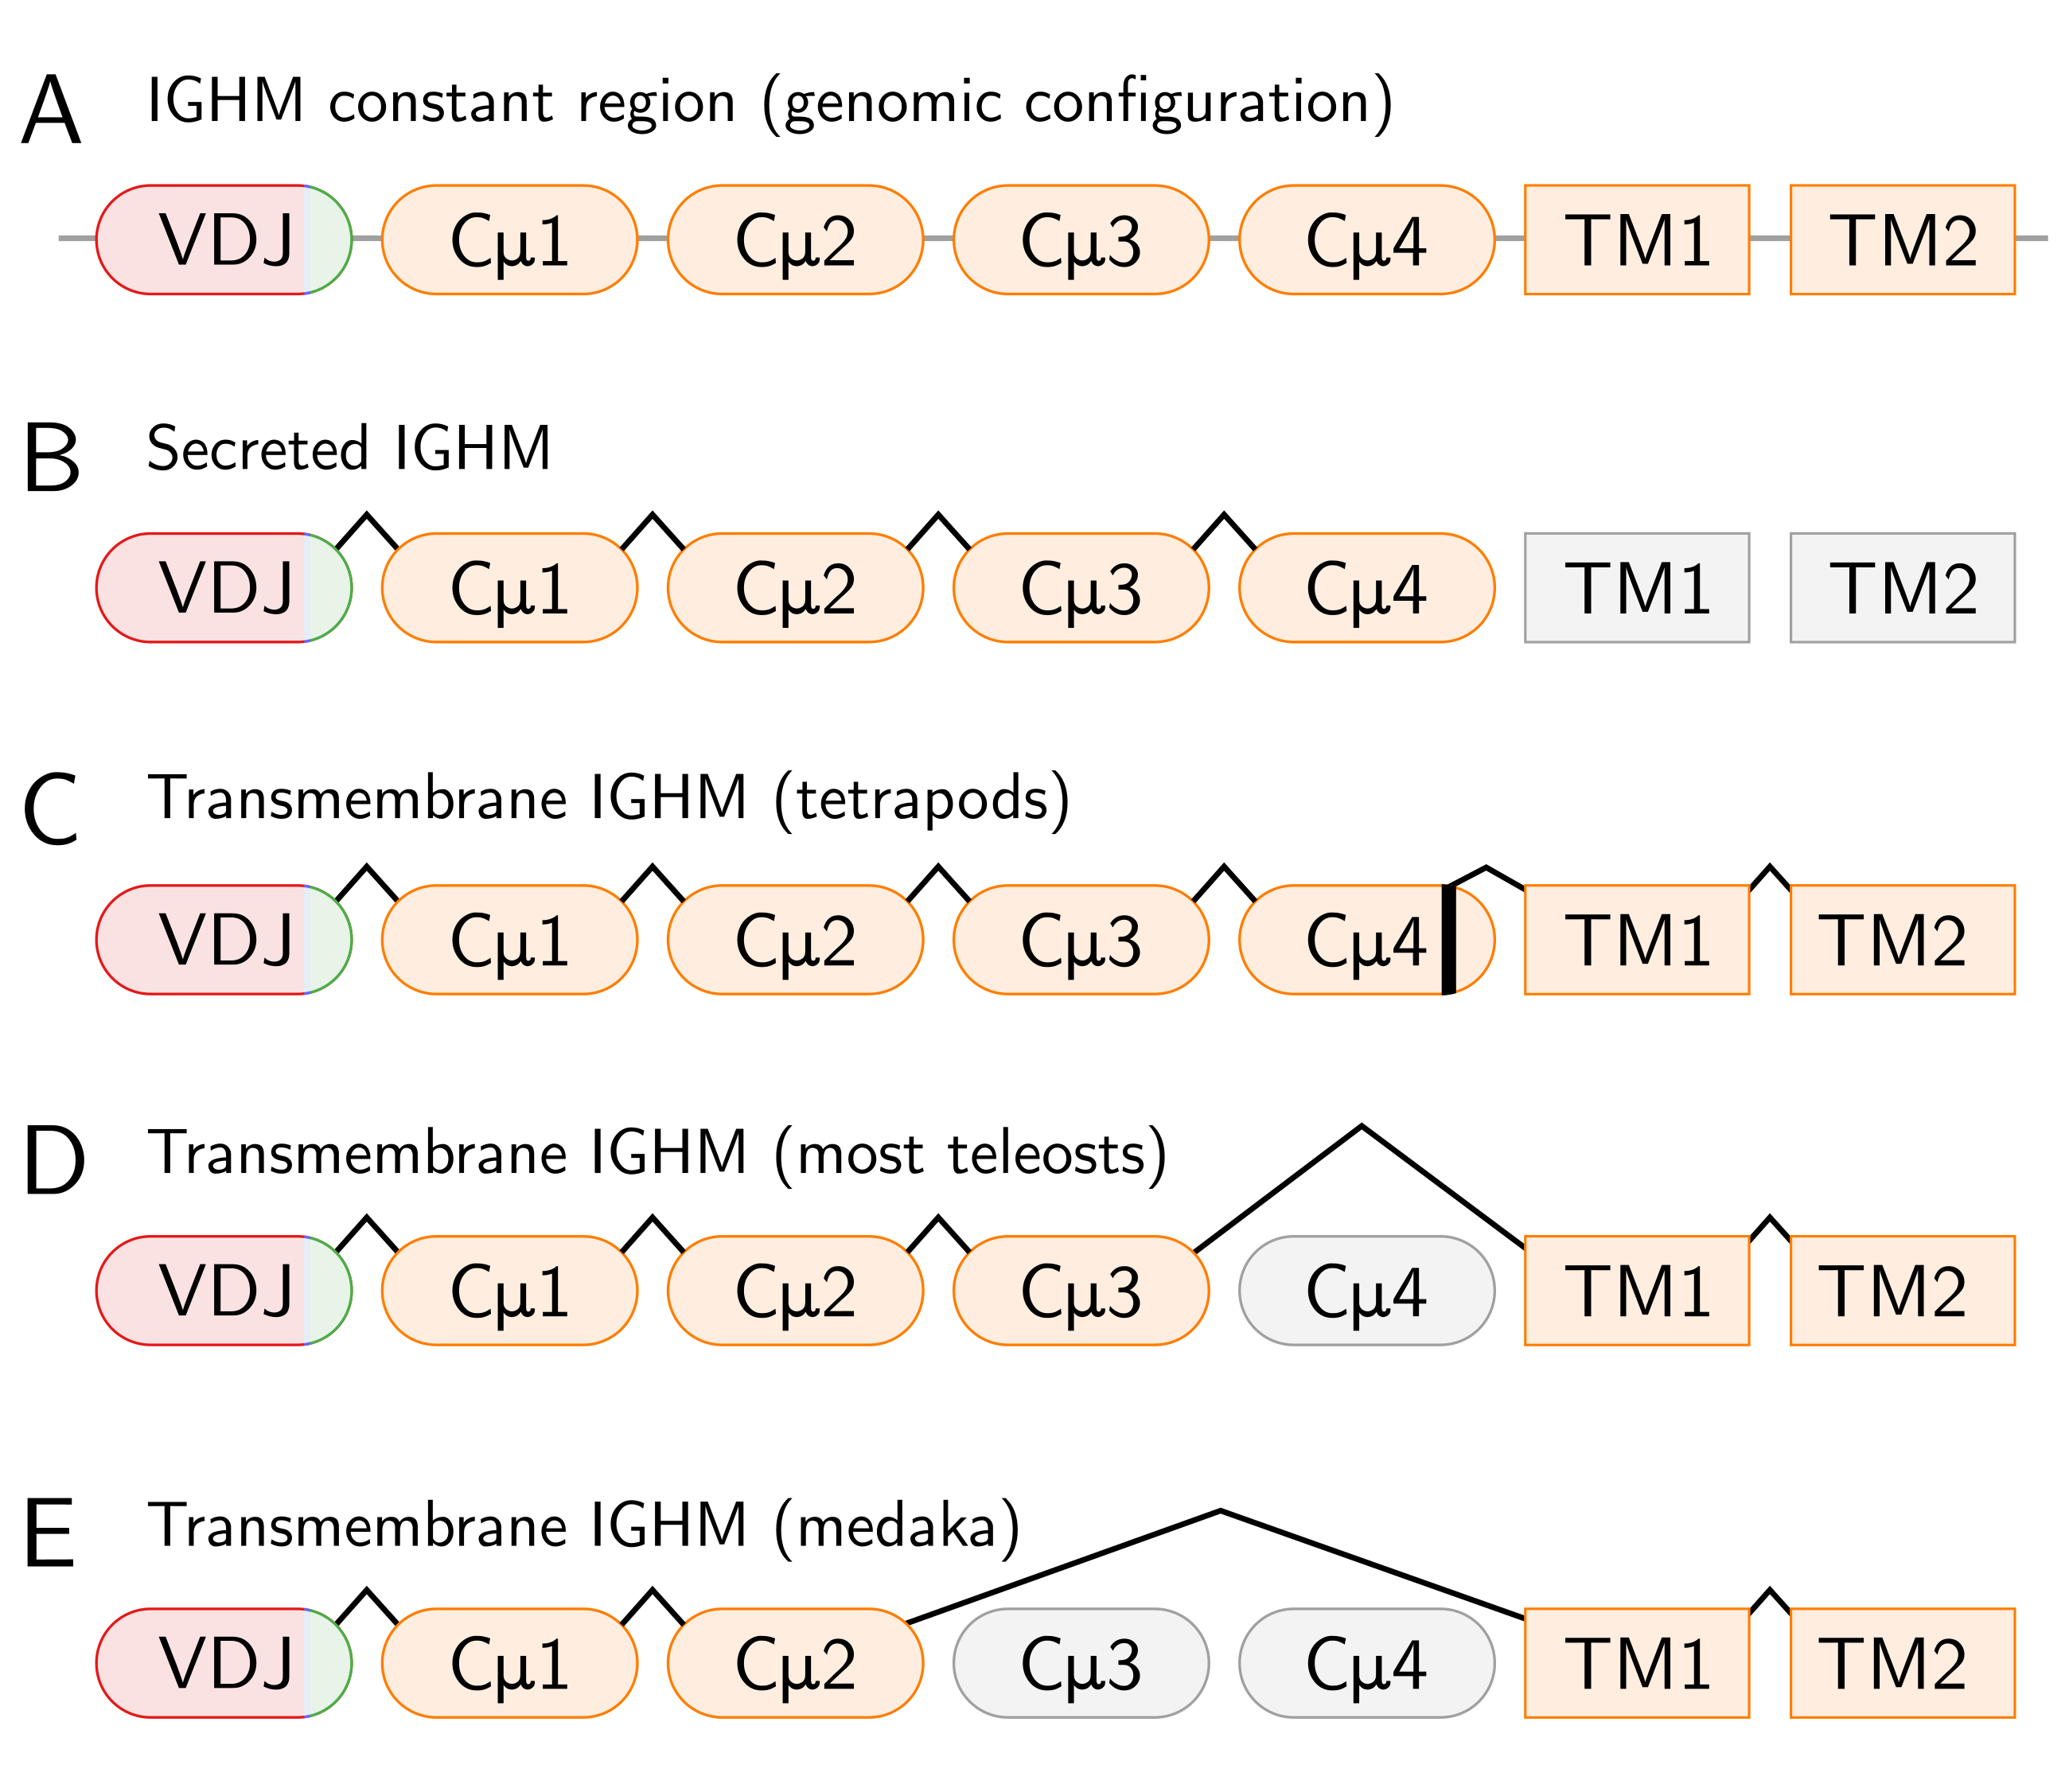
\includegraphics[width=0.8\textwidth]{_Figures/png_edited/teleost-igm-exons}
	\caption[\igh{M} exon usage in other vertebrates]{\textbf{\igh{M} exon usage in other vertebrates:} Schematic of \igh{M} splice patterns in different isoforms and taxonomic groups; (A) standard genomic (pre-splicing) configuration of \igh{M}, following VDJ recombination; (B) exon configuration of secreted \igh{M} (\igh{M-S}) in tetrapods and teleosts; (C) exon configuration of transmembrane \igh{M} (\igh{M-TM}) in tetrapods, demonstrating the use of a cryptic splice site in \cm{4}; (D) standard \igh{M-TM} exon configuration in teleosts, demonstrating the direct splicing of \cm{3} to TM1 and exclusion of \cm{4}; (E) unusual \igh{M-TM} exon configuration observed in medaka, in which both \cm{3} and \cm{4} are excluded. Figure adapted from Fillatreau \textit{et al.} (2013).}
	\label{fig:teleost-igm-exons}
	\end{figure}
	% TODO: Edit figure from IgM to IGHM
	
	\begin{figure}
	\centering
		\begin{subfigure}{0em}
        \phantomsubcaption{}
        \label{fig:nfu-locus-sashimi-a}
    \end{subfigure}
    \begin{subfigure}{0em}
        \phantomsubcaption{}
        \label{fig:nfu-locus-sashimi-b}
    \end{subfigure}
	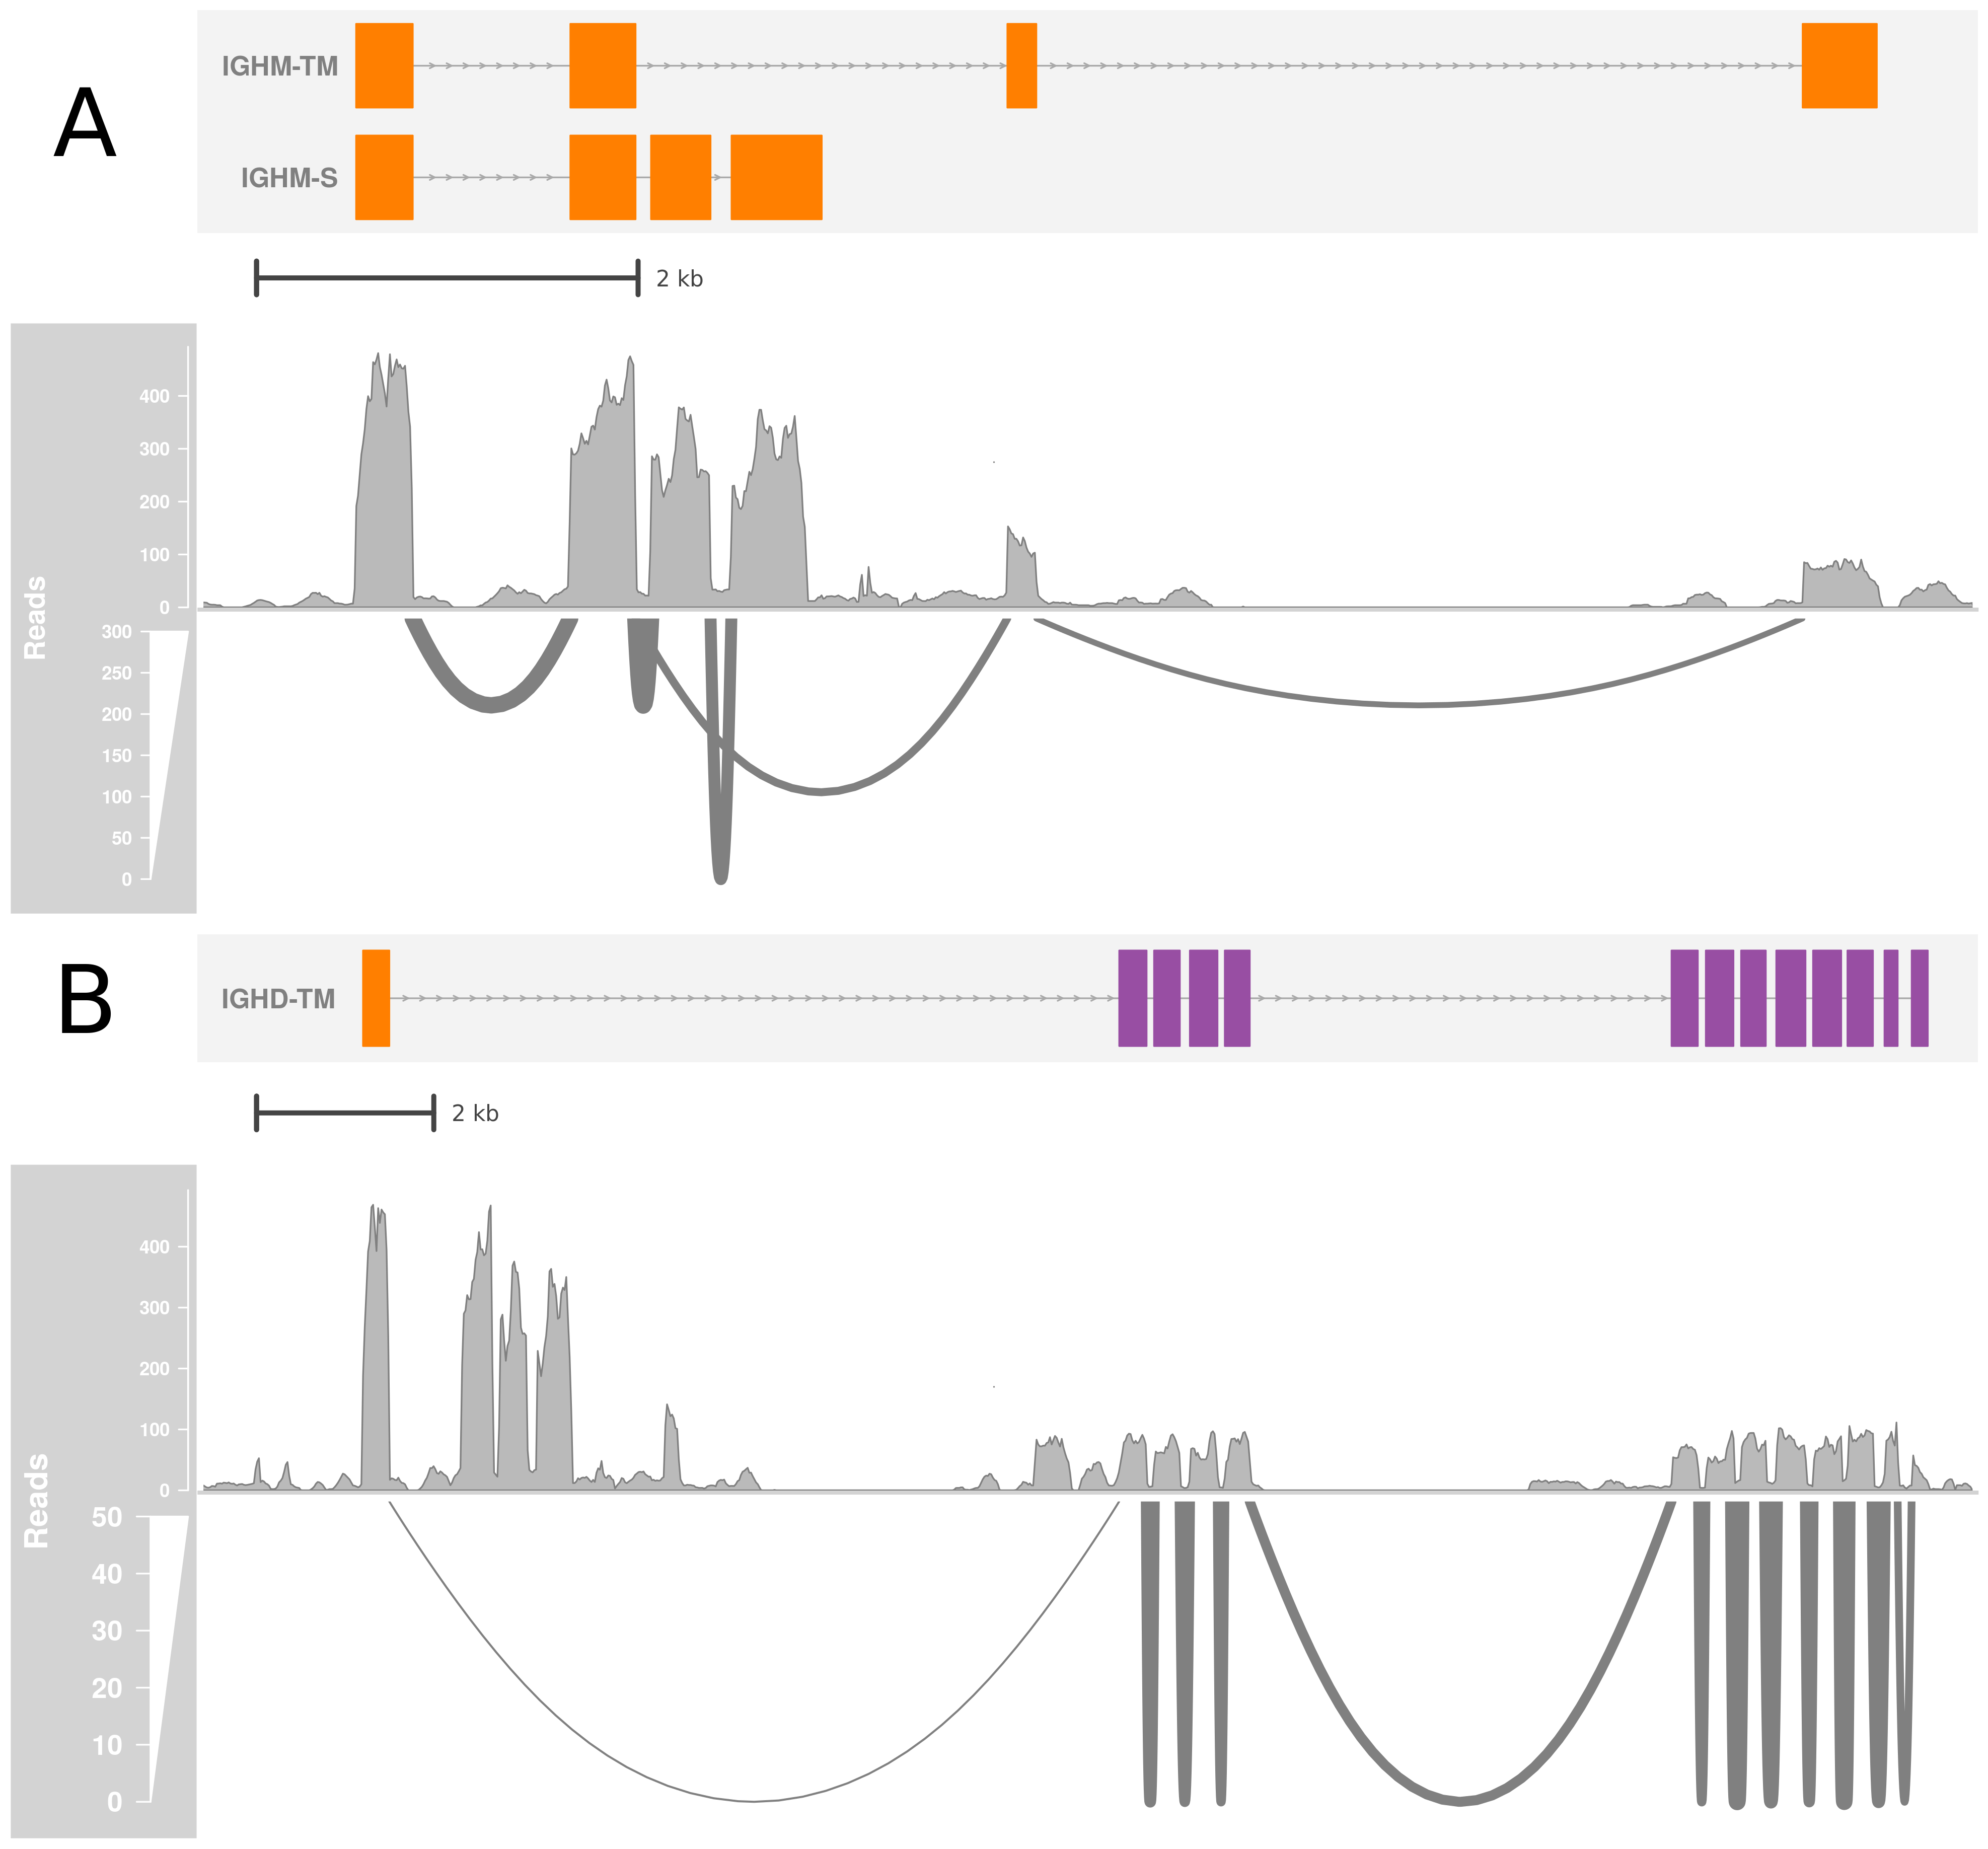
\includegraphics[width=\textwidth]{_Figures/png/nfu-locus-sashimi}
	\caption[Constant-region isoforms in \Nfu]{\textbf{Constant-region isoforms in \Nfu:} Coverage and sashimi plots of \program{STAR}-aligned RNA-seq reads from \Nfu gut samples \parencite{smith2017microbiota}, demonstrating the splicing behaviour of \igh{1} constant-region isoforms. (A) \igh{M} exon splicing, showing alternative splicing patterns of \igh{M-TM} and \igh{M-S}; (B) \igh{D} exon splicing, including chimeric splicing of \cm{1} to \cd{1}.}
	\label{fig:nfu-locus-sashimi}
	\end{figure}
	
	\begin{figure}
	\centering
	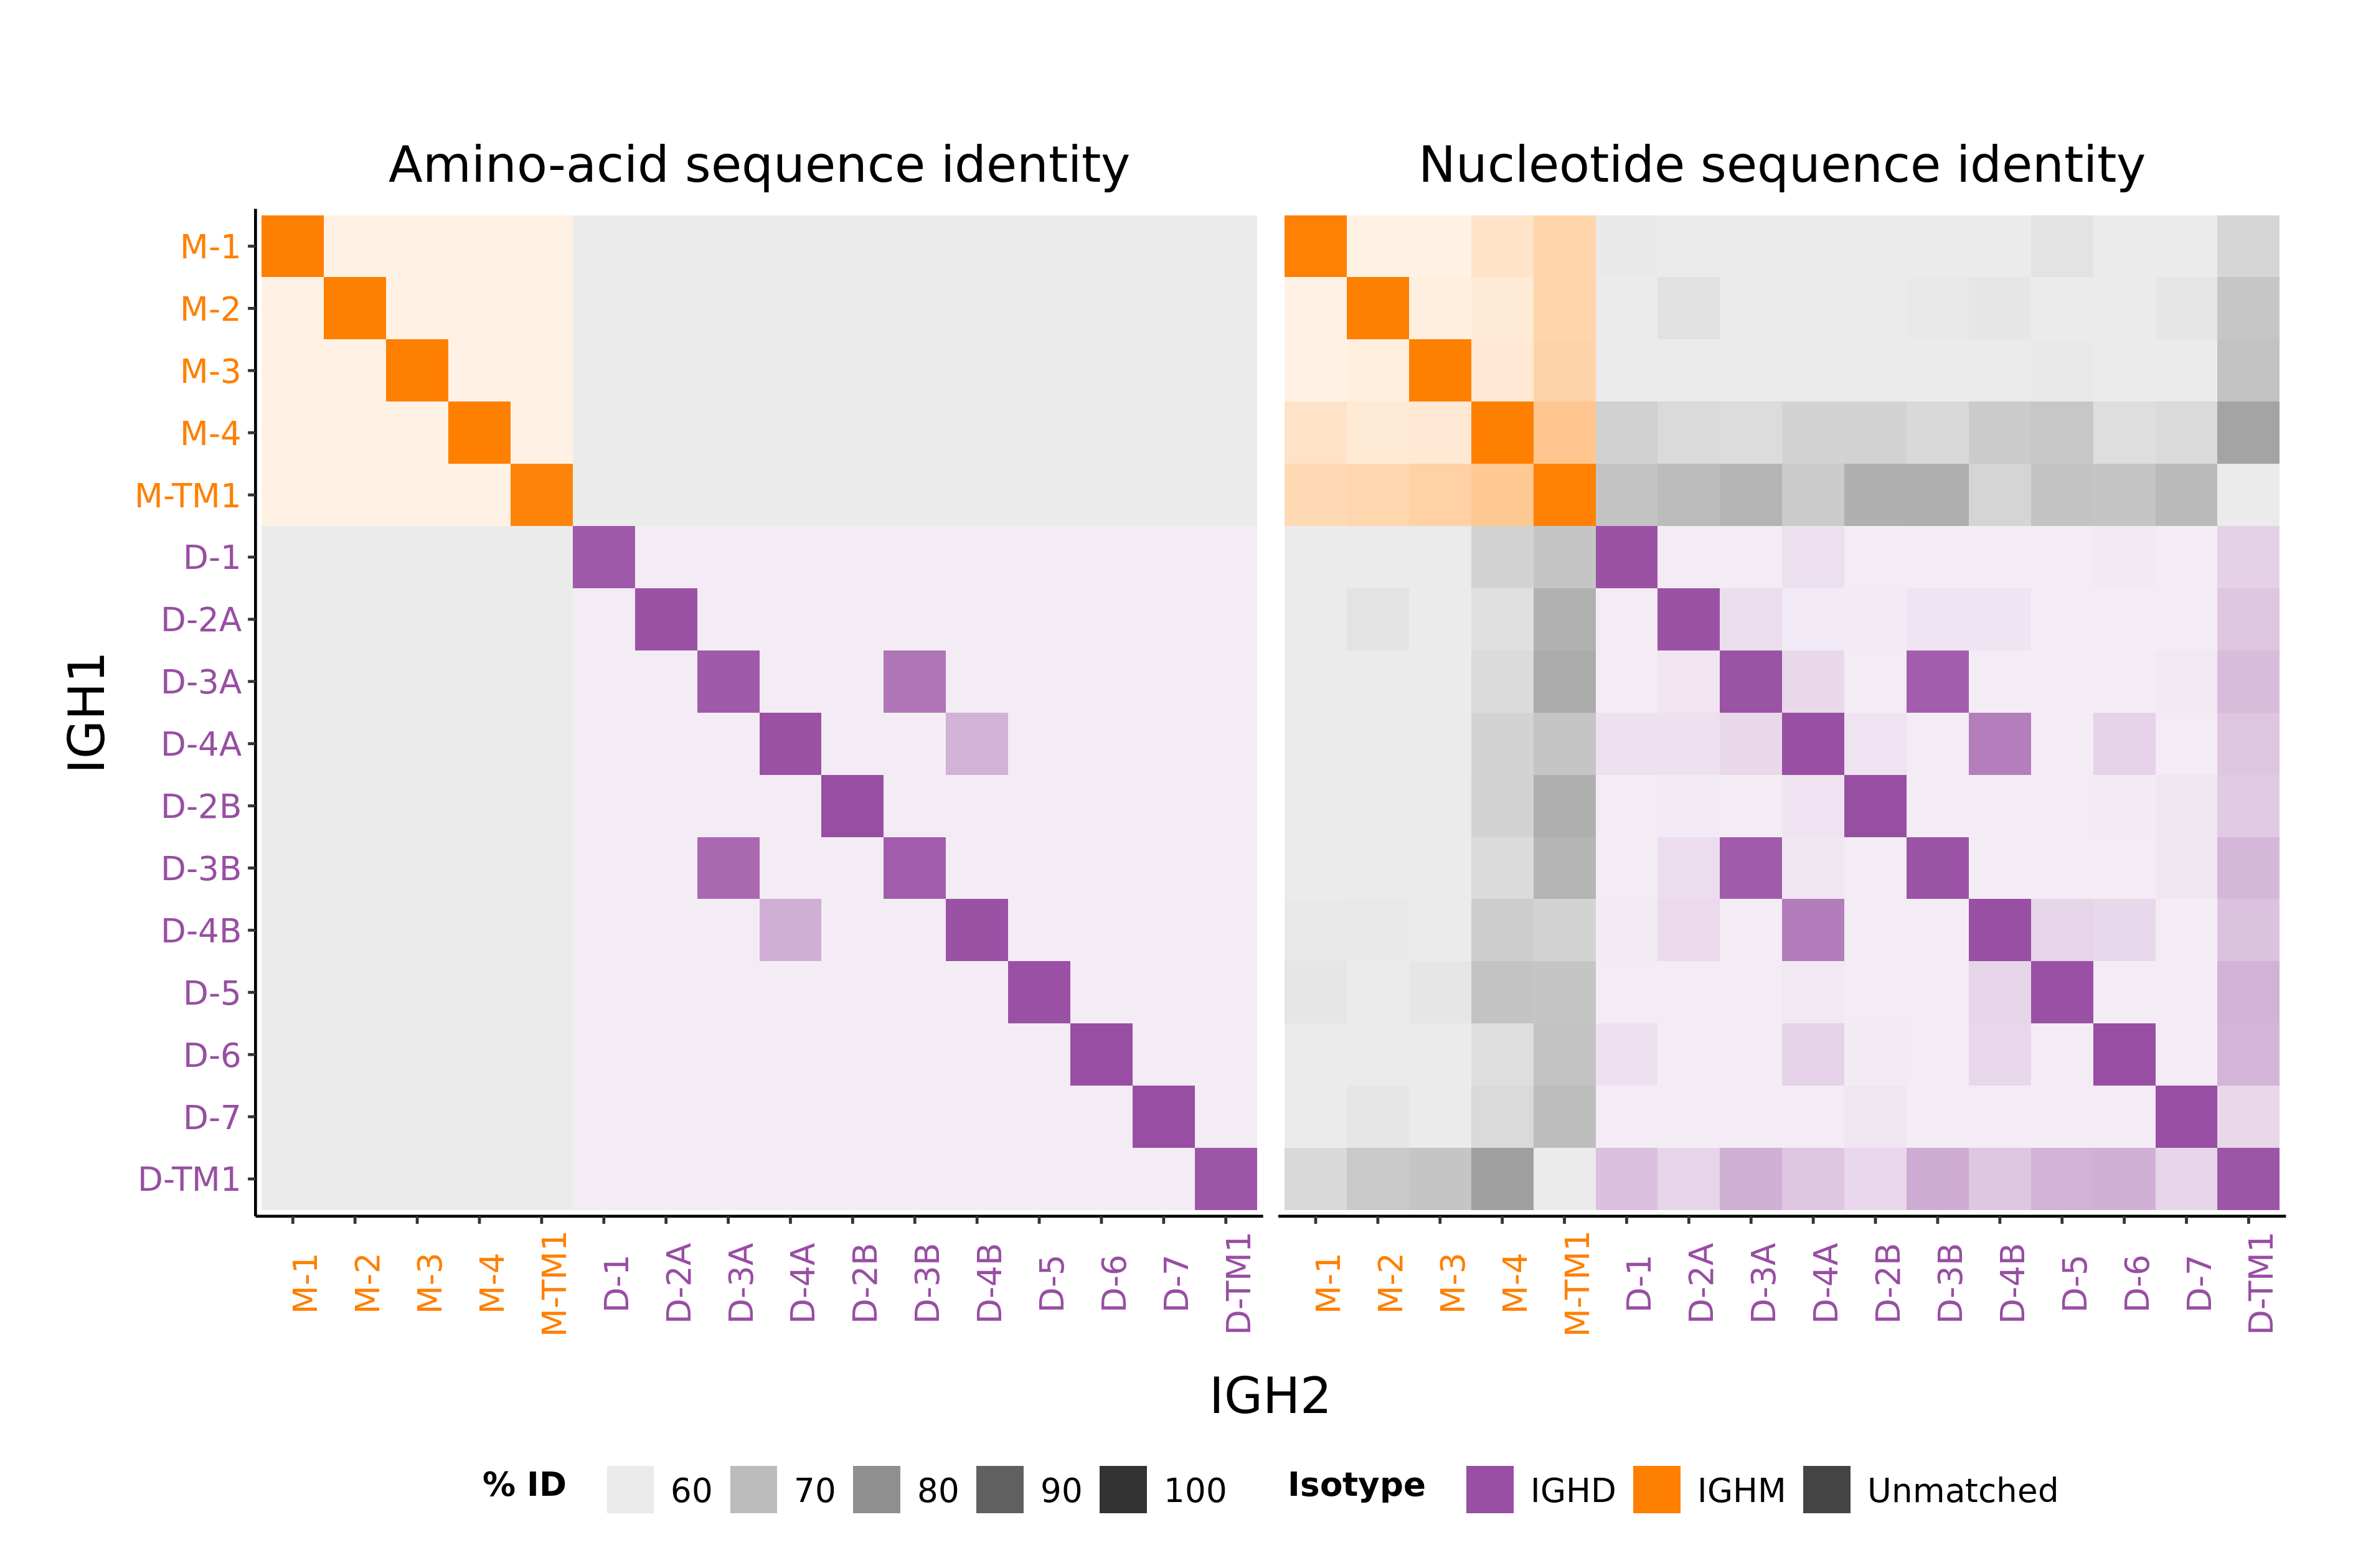
\includegraphics[width = \textwidth]{_Figures/png/nfu-ch-aln}
	\caption[Cross-sublocus sequence similarity in constant-region exons in \Nfu \textit{IGH}]{\textbf{Cross-sublocus sequence similarity in constant-region exons in \Nfu:} Heatmap of percentage sequence identity between amino-acid (right) and nucleotide (left) sequences of constant-region exons (excluding \igh{M-TM2} and \igh{D-TM2}) from the two subloci of \Nfu \textit{IGH}, calculated using pairwise Needleman-Wunsch global alignments..}
	\label{fig:nfu-ch-aln}
	\end{figure}
	
	\begin{table}\centering
		\caption[Cross-sublocus sequence similarity between corresponding constant-region exons in \Nfu \textit{IGH}]{\textbf{Cross-sublocus sequence similarity in constant-region exons in \Nfu:} Percentage sequence identities of pairwise Needleman-Wunsch global alignments between nucleotide (NT) or amino-acid (AA) sequences of corresponding exons from the two subloci of \Nfu \textit{IGH}.}
	% latex table generated in R 3.5.1 by xtable 1.8-3 package
% Wed Dec 19 17:33:43 2018
\begin{tabular}{llrr}
  \toprule Isotype & Exon & NT & AA \\ 
  \midrule M & 1 & 99.66 & 100.00 \\ 
  M & 2 & 100.00 & 100.00 \\ 
  M & 3 & 100.00 & 100.00 \\ 
  M & 4 & 100.00 & 100.00 \\ 
  M & TM1 & 99.34 & 98.00 \\ 
  M & TM2 & 91.67 & 100.00 \\ 
  D & 1 & 99.03 & 97.06 \\ 
  D & 2A & 98.97 & 98.96 \\ 
  D & 3A & 98.72 & 97.09 \\ 
  D & 4A & 99.65 & 98.92 \\ 
  D & 2B & 100.00 & 100.00 \\ 
  D & 3B & 98.72 & 96.12 \\ 
  D & 4B & 99.64 & 98.91 \\ 
  D & 5 & 99.09 & 99.08 \\ 
  D & 6 & 100.00 & 100.00 \\ 
  D & 7 & 100.00 & 100.00 \\ 
  D & TM1 & 97.99 & 97.96 \\ 
  D & TM2 & 99.44 & 100.00 \\ 
   \bottomrule \end{tabular}

	\label{tab:nfu-ch-aln}
	\end{table}
	
\subsection{Variable regions}
\label{sec:nfu-locus-variable}

\newabbreviation{EMBOSS}{EMBOSS}{European Molecular Biology Open Software Suite}
\newabbreviation{RNA-seq}{RNA-seq}{RNA sequencing}
\newabbreviation{TRB}{TRB}{T-cell receptor beta}
	
Variable-region gene segments in the killifish \igh{} locus were identified with a variety of methods, depending on the type of gene segment being analysed. \vh candidates were identified probabilistically using Hidden Markov Models constructed by \program{nhmmer} \parencite{wheeler2013nhmmer} from \program{PRANK} \parencite{loytynoja2014prank} multiple-sequence alignments of reference sequences, with the 3'-ends of each V-exon identified by the presence of a recombination-signal sequence (RSS) \parencite{schroeder2010immunoglobulins} and the 5'-ends refined using \program{IMGT-DomainGapAlign} \parencite{ehrenmann2011domaingapalign}. \jh candidates were also identified using \program{nhmmer}, with segment ends identified by the presence of an RSS (5') and a \sequence{GTA} splice-site motif (3') \parencite{magadan2011medaka}. Finally, \dh-segments, being too short and variable in sequence for HMM-based approaches to be effective, were identified by searching for pairs of flanking RSS sequences in opposite orientation, using fuzzy pattern-matching (with EMBOSS \program{FUZZNUC} \parencite{rice2000emboss}) to conserved RSS sequence motifs.
	 
In total, 24 \vh-segments, 14 \dh-segments and 17 \jh-segments were identified in the \Nfu locus (\Cref{tab:nfu-vh-coords,tab:nfu-dh-coords-seg,tab:nfu-jh-coords-seg}), of which the majority (17 \vh, 10 \dh and 8 \jh) were present in \igh{1}. Of the \vh segments identified, three contain premature STOP codons, though none is out-of-frame; conversely, all the \dh and \jh segments identified appear to be in-frame and functional, with no premature STOP codons. However, in all cases a minority of segments contain RSS sequences that deviate significantly from the expected consensus sequence (\Cref{tab:nfu-vh-coords,tab:nfu-dh-coords-rss5,tab:nfu-dh-coords-rss3,tab:nfu-jh-coords-rss}); it is unclear whether these sequences can recombine to successfully produce mature VDJ sequences \textit{in vivo}. In the case of the \vh segments, of the six sequences without clearly functional RSS sequences, three also contain premature STOP codons, suggesting the changes to the RSS in these cases may arise from relaxed purifying selection on already-pseudogenised sequences.

Apart from these few exceptions, however, the recombination signal sequences (RSS) marking the ends of the \vh, \dh and \jh gene segments in the \Nfu locus otherwise strongly resemble those of other characterised teleosts, which in turn resemble those of non-teleost loci (\Cref{fig:nfu-rss-seqlogo-all,fig:nfu-rss-seqlogo-sep}). The overall heptamer and nonamer consensus sequences (\texttt{CACAGTG} for heptamers and \texttt{ACAAAAACC} for nonamers) closely matched those expected from the literature \parencite{schroeder2010immunoglobulins}, while in 88\% of cases the spacer region was within 1bp of the expected length (12bp for D-RSSs, 23bp for V- and J-RSSs); unexpectedly, the greatest number of \vh-RSSs had a 22bp (rather than 23bp) spacer, but this is unlikely to interfere with RSS functionality. Overall, the RSSs in the turquoise killifish appear to be supporting the normal operation of VDJ-recombination in this species.

Of the \vh, \dh and \jh segments identified, all but one of each type of segment is located within contiguous V-, D-, and J-regions within each sublocus, supporting a modified translocon configuration for killifish \igh. The exceptions to this are \igh{1D01} and \igh{1J01}, which are embedded within the \igh{1} V-region, and a single \vh segment located in between the \igh{D} contant regions of the two subloci (\Cref{fig:nfu-locus-map-b}). The unusual location of \igh{1D01} and \igh{1J01} may represent the result of a transposition event within the \igh{} locus; however, their close colocalisation and 5' position within the \igh{1} sublocus, as well as the fact that neither has a close paralogue in \igh{2} (\Cref{fig:nfu-dj-alignment-b}), suggest that they may instead represent the remnant of a formerly present \igh{Z} constant region, as these typically have dedicated D/J segments independent of those serving \igh{M}. Given its forward orientation, meanwhile, the orphaned \vh-segment was assigned to the \igh{1} sublocus as \igh{1V1-07}; however, if annotated correctly, it is unlikely to successfully recombine with segments in either sublocus due to its unusual location.
		
\begin{table}[hb]
	\centering
	\begin{threeparttable}
	\centering
	\caption{Number of functional \vh-segments and \vh-families in other teleost species.}
	\label{tab:teleost-vh-counts}
	\begin{tabular}{ccccc}\toprule
	\multirow{2}{*}{	\textbf{Common Name}} & \multirow{2}{*}{\textbf{Species}} & \textbf{\# Functional} & \textbf{	\# \vh} & \multirow{2}{*}{\textbf{Source}} \\
	& & \textbf{\vh Segments} & \textbf{Families} & \\\midrule
	Zebrafish & \textit{Danio rerio} & 39 & 13\,\tnote{1} & \parencite{magadan2015fishrepertoires} \\
	Grasscarp & \textit{Ctenopharyngodon idella} & 8 & 5\,\tnote{2} & \parencite{xiao2010grasscarp} \\
	Fugu & \textit{Takifugu rubripes} & 34 & 3 & \parencite{magadan2015fishrepertoires} \\
	Medaka & \textit{Oryzias latipes} & 35 & 6 & \parencite{fillatreau2013astonishing,magadan2011medaka} \\
	Stickleback & \textit{Gasterosteus aculeatus} & 49 & 4 & \parencite{magadan2015fishrepertoires} \\
	Turquoise killifish & \textit{Nothobranchius furzeri} & 21\,\tnote{3} & 6 & -- \\
	\bottomrule\end{tabular}
	\begin{tablenotes}
	\item[1] \vh families in zebrafish identified based on 70\% (rather than 80\%) sequence identity.
	\item[2] It is not clear what clustering method or threshold was used to identify \vh families in grasscarp.
	\item[3] Excluding \vh segments with nonsense or frameshift mutations, but not those with uncertain or missing RSS sequences.
	\end{tablenotes}
	\end{threeparttable}
\end{table}
	
\vh sequences within an \igh{} locus are conventionally grouped into families on the basis of nucleotide sequence identity, with a typical identity cutoff of 80\% \parencite{magadan2015fishrepertoires}. In order to group the \Nfu \vh genes into families, pairwise Needleman-Wunsch global alignments were performed on each pair of \vh sequences to obtain pairwise identity scores, followed by single-linkage clustering on the resulting identity matrix. Cutting the dendrogram at 80\% sequence identity revealed a total of six \vh families, of which four contained more than one \vh segment (\Cref{fig:nfu-vh-families}); this number of \vh families in the \Nfu locus is roughly in line with those found in related species (\Cref{tab:teleost-vh-counts}). Of these, V1 and V2 make up the bulk (42\% and 29\% respectively) of the \vh segments in the locus. V2 and V4 are highly similar, and all the members of V4 are pseudogenised by premature STOP codons; it may therefore be more appropriate to regard V4 as a pseudogenised subfamily of V2 than as a \vh family in its own right.

The total number of functional \vh segments in the killifish locus is unusually small in comparison to the total numbers observed in many other teleost species (\Cref{tab:teleost-vh-counts}); however, the number of segments per sublocus is in line with the numbers seen in closely-related species (2 to 12 in medaka, 6 to 18 in stickleback), with the overall difference mainly arising from a difference in the number of subloci per locus. A similar pattern is observed with \dh and \jh segments, with similar numbers of segments per sublocus in killifish and closely-related species, especially medaka. It therefore appears that the per-sublocus segment diversity available to the turquoise killifish is similar to that of previously characterised species, with any difference in total available diversity at this level arising from differences in the number of functional subloci rather than the size of the V/D/J-regions \textit{per se}.

As can be seen from \Cref{fig:nfu-locus-synteny}, much of the V-, D- and especially J-region sequence in the \Nfu locus is syntenic between the two \igh{} subloci, with downstream portions of the \igh{2} V-region corresponding to downstream parts of the \igh{1} region. Of the seven \vh segments in \igh{2}, six have a correspending segment on \igh{1} with which they share at least 97\% sequence identity (\Cref{fig:nfu-vh-families}), and these partner segments are largely (though not entirely) colinear in their ordering between the two subloci. A similar pattern can be observed for the D- and (especially) the J-regions: of the four \dh segments detectable in \igh{2}, three (\igh{2D02} to \igh{2D04}) are identical with another block of adjacent \dh segments in \igh{1} (\igh{1D05} to \igh{1D07}), while the \jh-regions exhibit almost complete sequence identity between the eight \jh segments of the main \jh region in \igh{1} and the eight \jh segments in \igh{2} (\Cref{fig:nfu-dj-alignment}).
		
Nevertheless, as is clear from \Cref{fig:nfu-locus-synteny}, there are large portions the \igh{1} variable region, including the first 25 kilobases of the V-region, for which no corresponding sequence exists in \textit{IGH2}, and there are many \vh and \dh segments in \igh{1} (and a much smaller number in \igh{2}) for which no close homologue exists in the other sublocus. Taken together, these data are consistent with a model in which \igh{2} was produced via duplication and inversion of all or part of \igh{1}, followed by subsequent deletion events in the redundant, and structurally volatile, \igh{2} \vh and \dh regions. However, it is not clear at present how to distinguish between this model and an alternative one of expansion in \igh{1}, or to identify why the \jh region is so much more conserved between subloci than either the \vh or \jh regions.

	
	\begin{figure}
	\centering
	\begin{subfigure}{0em}
	\phantomsubcaption{}
    \label{fig:nfu-vh-families-a}
    \end{subfigure}
    \begin{subfigure}{0em}
    \phantomsubcaption{}
    \label{fig:nfu-vh-families-b}
    \end{subfigure}
	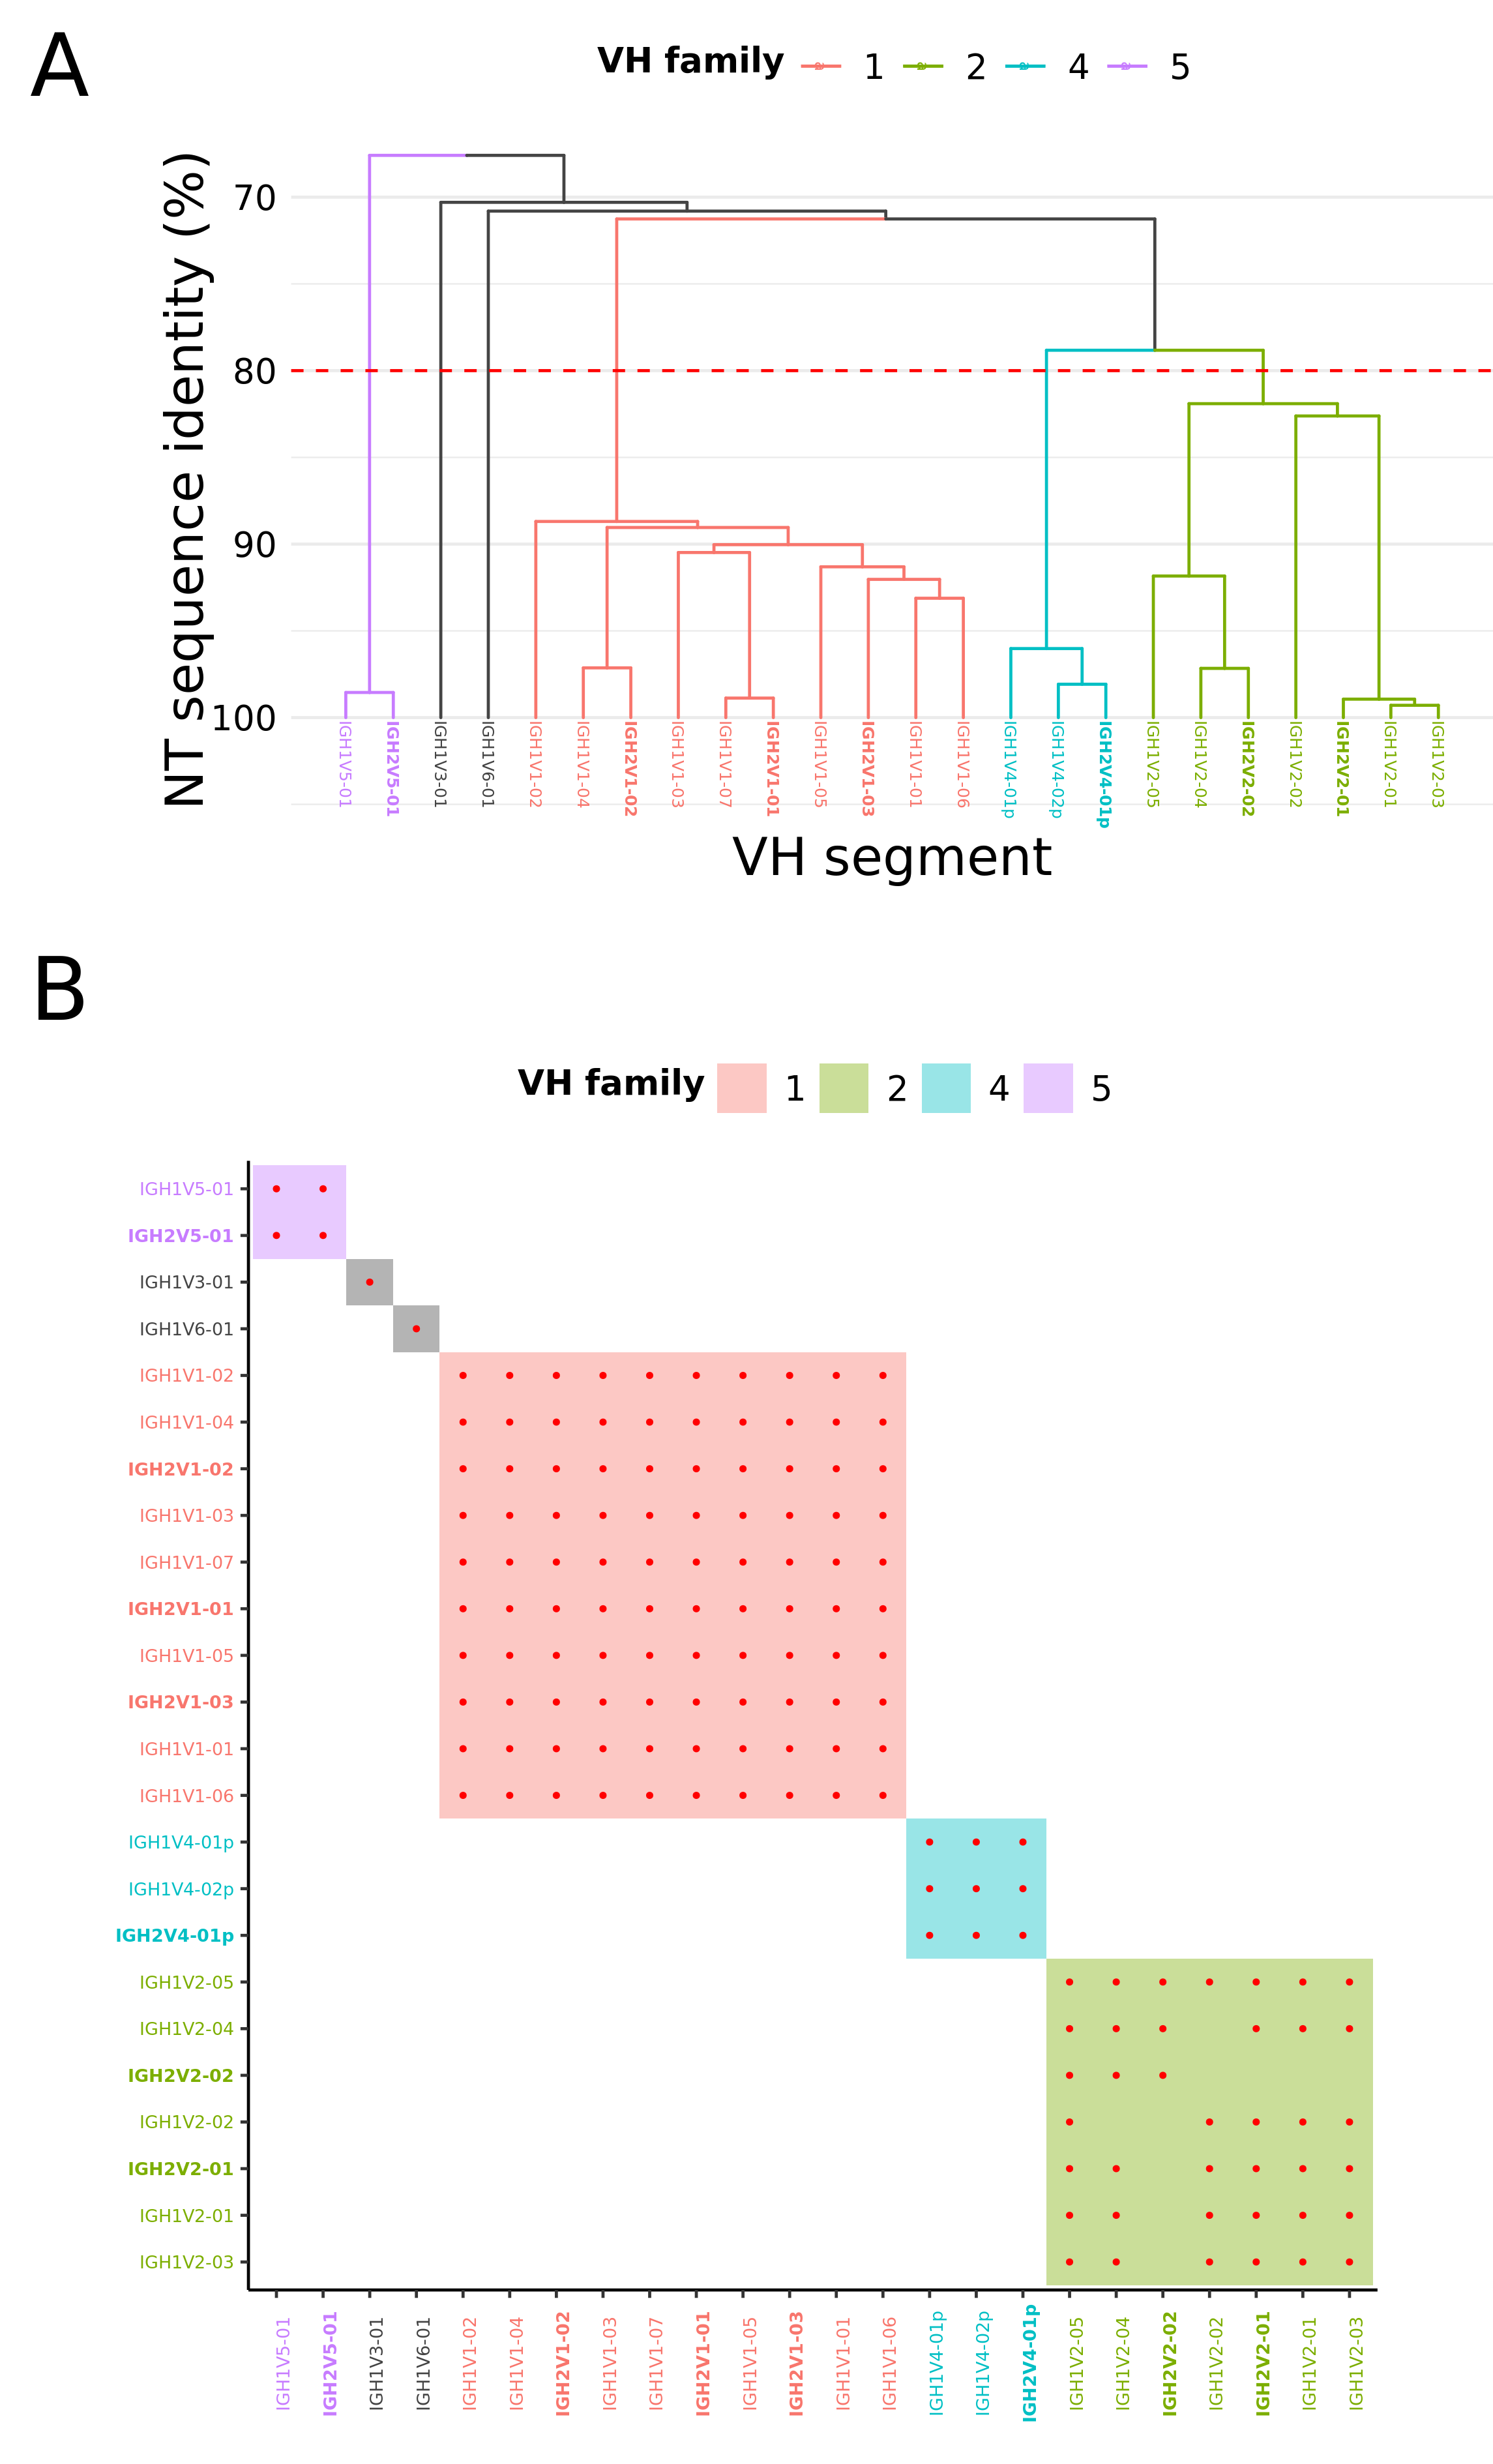
\includegraphics[width=0.8\textwidth]{_Figures/png/nfu-vh-families.png}
	\caption[\vh families in the in \Nfu \igh{} locus]{\textbf{\vh families in the in \Nfu \igh{} locus:} (A) Dendrogram of sequence similarity of \vh segments in the \Nfu \igh{} locus, arranged by single-linkage clustering on nucleotide sequence identity. The red line indicates the 80\% cutoff point for family assignment, while branch colour indicates family membership. (B) Heatmap of family relationships among \Nfu \vh segments, with coloured shading indicating families and red dots indicating pairwise nucleotide sequence identity of at least 80\%. In both subfigures, \vh families containing multiple segments are coloured, single-segment families are in grey, and segments from the \igh{2} sublocus are displayed in \textbf{boldface}.}
	\label{fig:nfu-vh-families}
	\end{figure}

\begin{figure}
\centering
	\centering
	\begin{subfigure}{0em}
	\phantomsubcaption{}
    \label{fig:nfu-dj-alignment-a}
    \end{subfigure}
    \begin{subfigure}{0em}
    \phantomsubcaption{}
    \label{fig:nfu-dj-alignment-b}
    \end{subfigure}

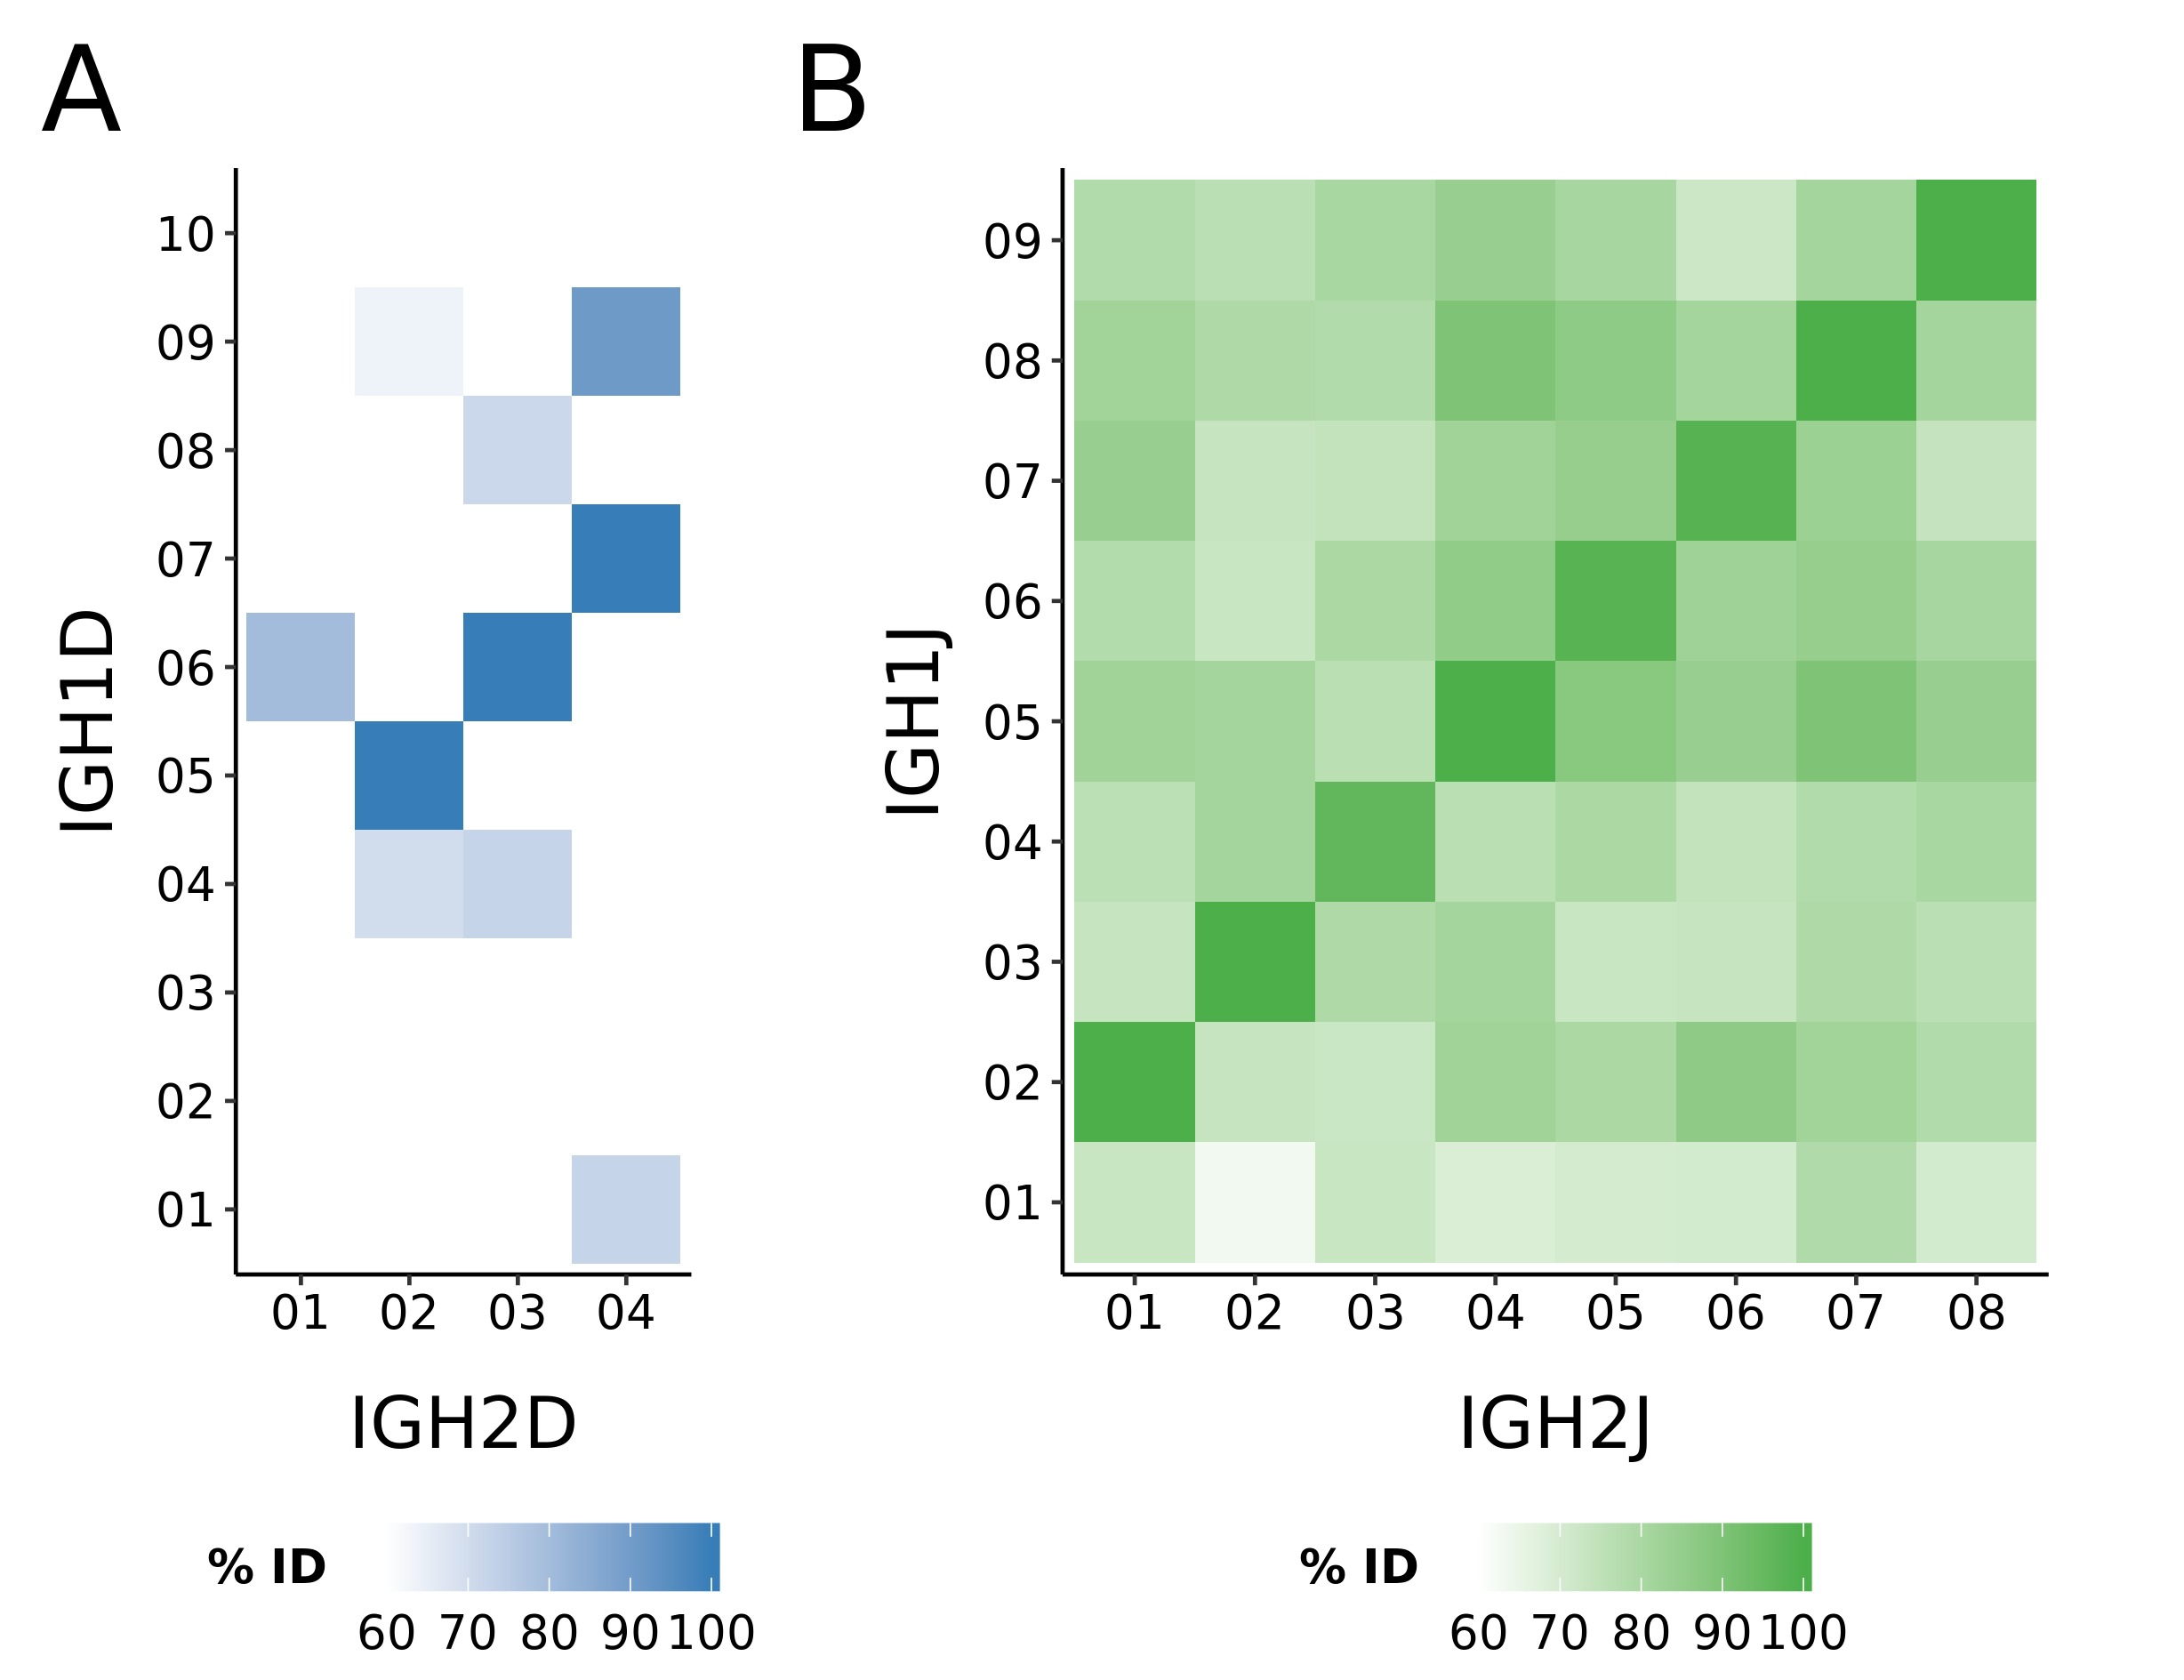
\includegraphics[width=0.6\textwidth]{_Figures/png/nfu-dj-aln}
\caption[Cross-sublocus sequence similarity in \dh and \jh gene segments in \Nfu]{\textbf{Cross-sublocus sequence similarity in \dh and \jh gene segments in \Nfu:} Heatmap of percentage nucleotide sequence identities of Needleman-Wunsch global alignments between (A) \dh and (B) \jh gene segments in IGH1 vs IGH2, revealing syntenic runs of highly similar sequences across both subloci.}
\label{fig:nfu-dj-alignment}
\end{figure}	
	
	\begin{figure}
	\centering
	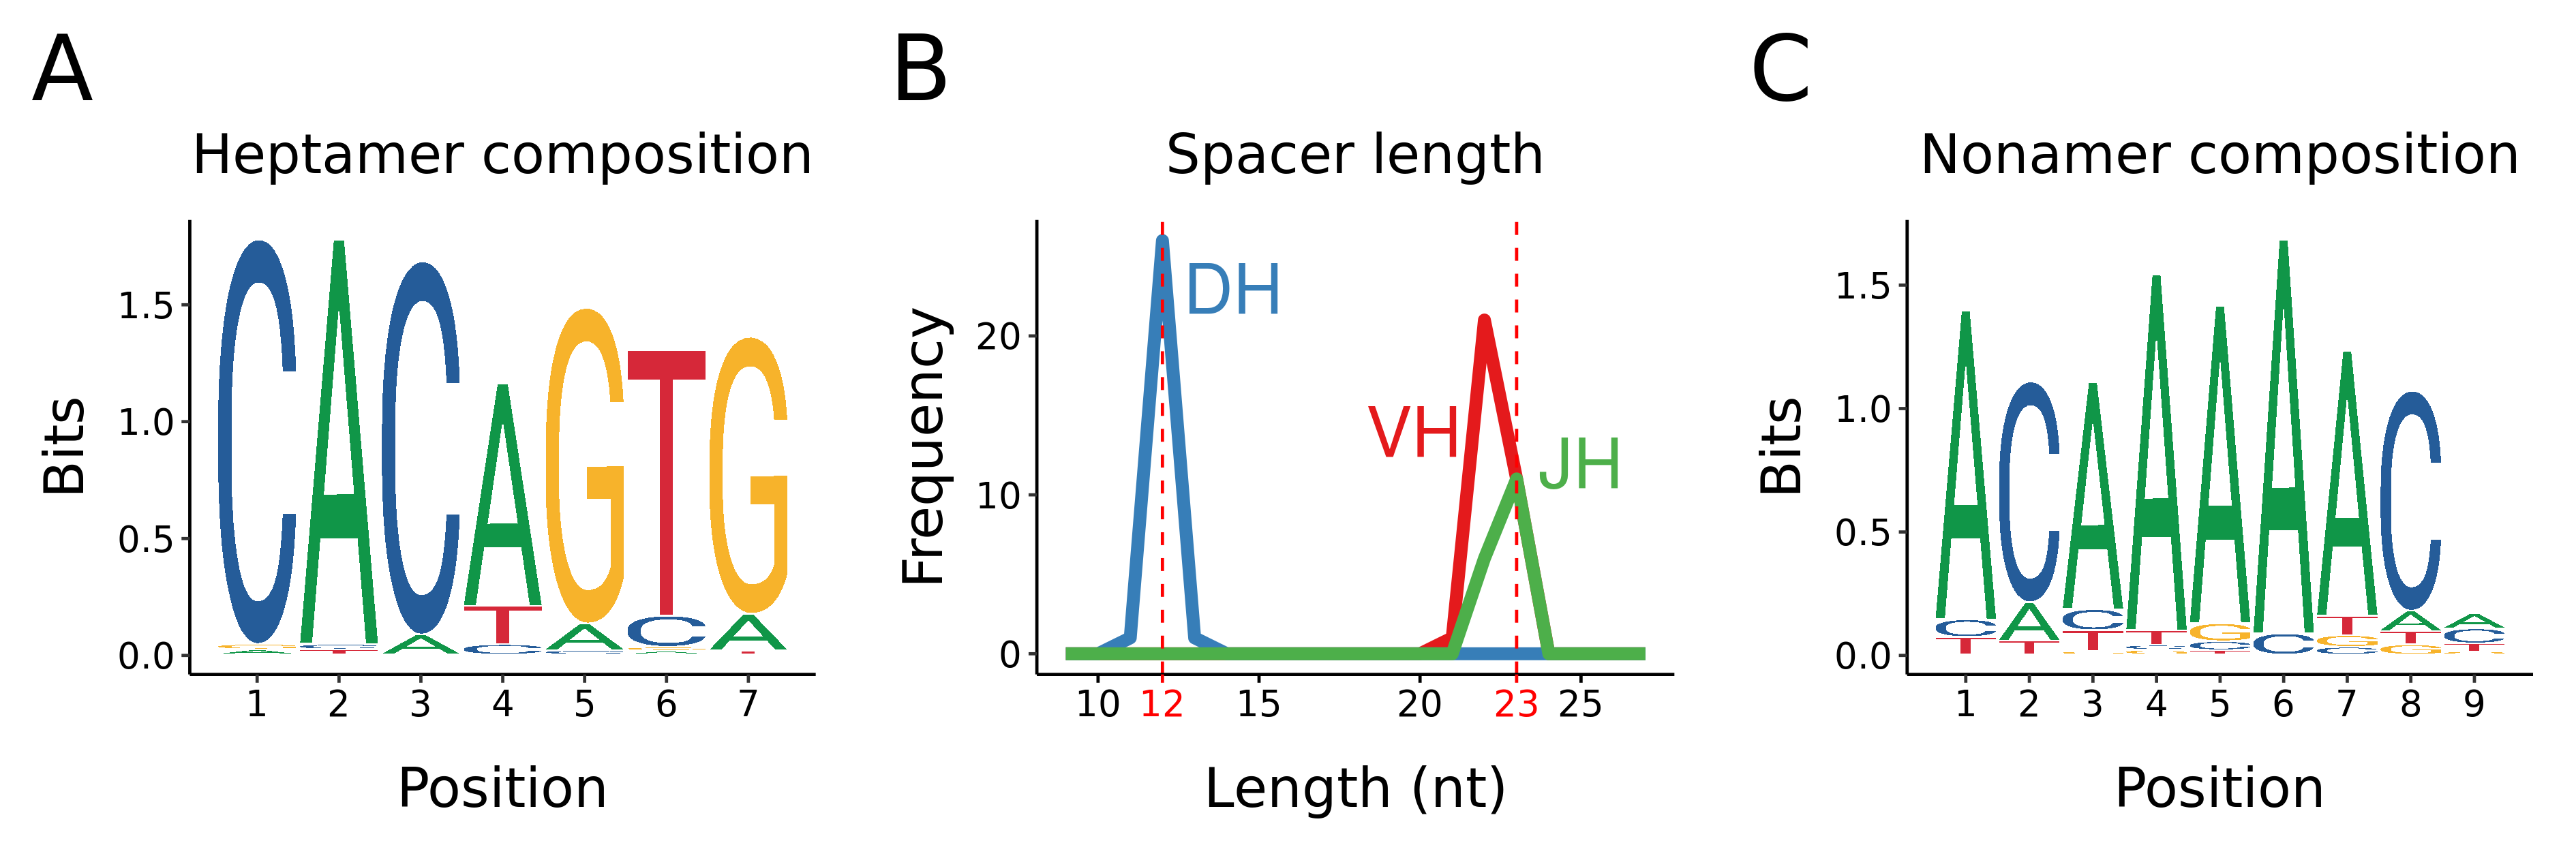
\includegraphics[width=\textwidth]{_Figures/png/nfu-rss-seqlogo-all}
	\caption[Recombination signal sequences in the \Nfu \textit{IGH} locus]{\textbf{Recombination signal sequences in the \Nfu \textit{IGH} locus:} (A) Sequence composition of conserved heptamer sequences across all \Nfu heavy-chain RSSs; (B) length distribution of unconserved spacer sequences in \Nfu heavy-chain RSSs; (C) sequence composition of conserved heptamer sequences across all \Nfu heavy-chain RSSs.}
	\label{fig:nfu-rss-seqlogo-all}
	\end{figure}
	
\FloatBarrier



\clearpage